\documentclass[preprint,3p,times]{elsarticle}
% TO Read:
% 删除文本包含在命令里
% 替换文本在\red{}里

\usepackage{example}
% new environment
\usepackage{tabularray}
\usepackage{xcolor}
\graphicspath{{images/}}
\newcommand{\revise}[1]{\textcolor{blue}{#1}}
\newcommand{\norm}[1]{\left\lVert #1\right\rVert}
\newcommand{\abs}[1]{\left\lvert #1\right\rvert}
\newcommand{\Var}{\operatorname{Var}}
\newtheorem{proposition}{Proposition}[section]
% \newtheorem*{proof}{Proof}
%PolyU
\def\al{\alpha}
\def\fy{\varphi}
\def\x{\mathbf{x}}
\def\apriori{\textit{a priori }}
\def\L{\mathcal{L}}
\def\N{\mathcal{N}}
\def\B{\mathcal{B}}
\def\A{\mathcal{A}}
\def\I{\mathcal{I}}
\def\E{\mathbb{E}}

\def\S{\mathcal{S}}
\def\D{\mathcal{D}}
\def\Q{\mathcal{Q}}
\def\l{\ell}
\def\al{\alpha}
\def\dta{\partial_t^\alpha}
\def\d{\mathrm{d}}
\def\btau{\bar\partial_\tau^\al}

\begin{document}




\begin{frontmatter}


% \title{Transformed Monte Carlo fPINNs: Enhancing Computational Efficiency for Time-Fractional Diffusion-Wave Equations}
\title{Transformed Diffusion-Wave fPINNs: Enhancing Computational Efficiency for Time-Fractional Diffusion-Wave Equations}
\author[1]{Zhengqi Zhang}
\ead{zhengqizhang@zhejianglab.org}
\author[1]{Jing Li\corref{cor1}}
\ead{lijing@zhejianglab.org}
\cortext[cor1]{Corresponding author}
\affiliation[1]{organization={Zhejiang Lab}, city={Hangzhou}, postcode={311121},country={China}}
\begin{abstract}
We propose Transformed Diffusion-Wave Fractional Physics-Informed Neural Networks (tDWfPINNs) for efficiently solving time-fractional diffusion-wave equations with fractional order $\alpha \in (1, 2)$. Conventional numerical methods for these equations often compromise the mesh-free advantage of Physics-Informed Neural Networks (PINNs) or impose high computational costs when computing fractional derivatives. The proposed method avoids first-order derivative calculations at quadrature points by introducing a specific integrand transformation, effectively transferring the derivative operation from the solution to a smoother kernel. This redistribution of the derivative significantly reduces the computational overhead of automatic differentiation while preserving accuracy. \revise{We further establish consistency of the transformed operator, removable endpoint singularities, representation-level stability, and quadrature error estimates for both Monte Carlo and Gauss-Jacobi implementations.} We conduct a comprehensive comparative analysis of the proposed transformation using both Monte Carlo and Gauss-Jacobi quadrature across various time-fractional PDEs. Our results demonstrate that tDWfPINNs achieve superior computational efficiency without sacrificing accuracy. Furthermore, we incorporate the proposed approach into adaptive sampling approaches such as the residual-based adaptive distribution (RAD) for the time-fractional Burgers equation with order $\alpha \in (1, 2)$, which exhibits complex solution dynamics. The experiments show that the Gauss-Jacobi method typically outperforms the Monte Carlo approach; however, careful consideration is required when selecting the number of quadrature points. Overall, the proposed tDWfPINNs offer a significant advancement in the numerical solution of time-fractional diffusion-wave equations, providing an accurate and scalable mesh-free alternative for challenging fractional models.
\end{abstract}
  \begin{keyword}
    Physics Informed Neural Networks \sep Time-fractional Partial Differential Equations \sep Diffusion-wave
\end{keyword}


\end{frontmatter}


\section{Introduction}
\label{sec:intro}

In recent years, fractional and nonlocal models have attracted considerable interest owing to their broad applications in diverse disciplines, including physics, engineering, biology, and finance. Time-fractional diffusion-wave equations \eqref{def:pde}, in particular, have been extensively used to model the propagation of mechanical waves in viscoelastic media \cite{Mainardi1996, Mainardi2022}. Furthermore, such equations are instrumental in modeling the fractional dynamics of systems relevant to medicine \cite{Swain2025, BenSalah2025}. For a comprehensive overview of the applications of fractional models in biology and physics, readers are referred to \cite{Metzler2000, Metzler2014}.

Nevertheless, solving time-fractional diffusion-wave equations presents significant challenges, primarily stemming from their inherent nonlocality and wave-like characteristics. Analytical solutions involving Mittag-Leffler and Wright functions have been introduced in \cite{Sakamoto2011, Jiang2012, Agrawal2002}. To overcome these difficulties, a variety of numerical methods have been developed, including finite-difference methods \cite{Du2010, Sun2020}, convolution-quadrature methods \cite{Cuesta2006, Jin2017Correction}, collocation-type methods \cite{Zhu2019, Stynes2017}, and spectral methods \cite{Chen2020, Zayernouri2013}.

In recent years, the rapid advancement of computing resources and machine learning methodologies has brought Physics-Informed Neural Networks (PINNs) \cite{RaissiParisGE:2019:JCP, CaiMaoWangYinGE:2021:fluid, Cuomo2022:PINN:review} to the forefront of scientific computing. PINNs have attracted considerable attention due to their efficacy in solving PDEs, particularly benefiting from their mesh-free formulation, which alleviates the curse of dimensionality. To address the computational challenges associated with incorporating fractional derivatives into the PINNs framework, various numerical approximation techniques have been proposed. Among these, the fractional Physics-Informed Neural Networks (fPINNs), as proposed in \cite{Pang2019:fPINN}, have been widely adopted. The core strategy of fPINNs involves applying automatic differentiation for integer-order operators, while approximating fractional derivatives using numerical discretization schemes-typically based on finite difference-applied to the neural network outputs. For further developments in this direction, readers are referred to \cite{Lu2025, Vats2024}.

Despite their practical utility, these finite-difference-based schemes for fractional derivatives inherently rely on discretization grids, thereby compromising the mesh-free advantages that distinguish PINNs. Recent theoretical investigations \cite{Ren2023, WangYuParis:2022:NTK} have shown that PINNs exhibit a hierarchical spectral bias: they preferentially learn the low-frequency components of the solution, while accurate resolution of high-frequency features is delayed. This spectral bias imposes significant challenges in accurately capturing multiscale dynamics and motivates the development of advanced training strategies, such as adaptive sampling methods \cite{LuLu:2023:RAD, Zhang2025}. Building upon these advances, the present study proposes a fully mesh-free computational framework for the treatment of fractional derivatives, preserving the core advantages of PINN-based approaches.

Spectral methods \cite{Zhang2025Spectral, Chen2025} have been proposed to reformulate problems involving fractional derivatives by transforming the original time-space domain into the frequency domain. Although this approach effectively avoids direct numerical evaluation of fractional operators, it typically incurs elevated computational costs and may suffer from reduced accuracy due to the inverse transform. Alternatively, Monte Carlo fractional Physics-Informed Neural Networks (MCfPINNs) \cite{Guo2022:MCfPINN} leverage stochastic sampling to approximate both temporal and spatial fractional derivatives. Building on this framework, recent studies \cite{Hu2024:CMAME, Lin2025} have introduced Gauss-Jacobi quadrature rules to improve computational efficiency by replacing Monte Carlo integration with stochastic quadrature rules. Notably, both the Monte Carlo and the Gauss-Jacobi quadrature approaches can be seamlessly integrated into adaptive sampling frameworks, preserving the mesh-free character of PINN-based approaches and making them particularly well-suited for applications in fractional-order modeling within machine learning frameworks.

In this work, we consider an initial-boundary value problem of diffusion-wave equation with order $\alpha \in (1, 2)$:
\begin{equation}
    \label{def:pde}
    \begin{aligned}
        \dta u(t,\x) + \N(u(t,\x),f(t,\x)) &= 0,~~ (t,\x)\in (0,T]\times\Omega,\\
        u(t,\x)&=0,~~(t,\x)\in(0,T]\times\partial\Omega\\
        u(0,\x)=a(\x),\partial_tu(0,\x)&=b(\x), ~~\x\in\Omega,
    \end{aligned}
\end{equation}
where $T>0$ denotes the final time, and $\Omega\subset\mathbb{R}^d$ ($d=1,2,3$) is a convex polyhedral domain with boundary $\partial\Omega$. $\N$ is a time-independent differential operator acting on the solution $u$ and the source term $f$. $\dta u $ denotes the Caputo fractional derivative of order $\al \in (1, 2)$ with respect to time $t$, defined as \cite[P. 70]{Kilbas2006},
\begin{equation}
    \label{def:dtal}
    \dta u(t) = \frac{1}{\Gamma(2-\al)}\int_0^t (t-\tau)^{1-\al}\frac{d^2}{d\tau^2} u(\tau)\d\tau,
\end{equation}
where $\Gamma$ denotes the Gamma function.

In recent years, various PINNs-based methods have been proposed to address diffusion-wave problems. For example, \cite{Vats2024} employed fPINNs to solve time-dependent diffusion-wave equations, while Lu et al. \cite{Lu2025} utilized the $L2$ scheme to approximate Caputo fractional derivatives for $\alpha\in(0,2)$. Chen et al. \cite{Chen2025} applied the Laplace transform to reformulate the problem described by \eqref{def:pde}, and Lin et al. \cite{Lin2025} integrated tensor neural networks with Gauss-Jacobi quadrature to achieve high-accuracy estimation. Nevertheless, there remains a significant gap in the development of mesh-free methods for computing fractional derivatives of order $\alpha \in (1, 2)$. A commonly adopted approach is to extend the MCfPINNs framework-originally proposed for $\alpha\in(0,1)$-using either the Monte Carlo (MC) method \cite{Guo2022:MCfPINN} or Gauss-Jacobi (GJ) quadrature \cite{Hu2024:CMAME}.  However, simply extending the methodologies from \cite{Hu2024:CMAME,Lin2025} to diffusion-wave equations with order $\alpha \in (1, 2)$ encounters a critical computational bottleneck. Existing Gauss-Jacobi approaches \cite{Hu2024:CMAME,Lin2025} predominantly focus on problems where $\alpha \in (0, 1)$ or directly approximate the integral definition. When applied to $\alpha \in (1, 2)$, the standard Caputo definition involves the convolution of a singular kernel with the first-order derivative of the solution. Consequently, during the training of PINNs, the automatic differentiation engine is forced to construct a computational graph for the derivative at every single quadrature point. For $N$ training samples and $M$ quadrature points, this results in a computational complexity involving $O(MN)$ Hessian-vector product operations, which is prohibitively expensive in terms of both GPU memory and training time.




To address the aforementioned challenges, we propose transformed Diffusion-Wave fractional Physics-Informed Neural Networks (tDWfPINNs). The distinct novelty of our work compared to \cite{Hu2024:CMAME,Lin2025} lies in a strategic integrand transformation. Instead of directly discretizing the definition, we theoretically restructure the fractional operator using integration by parts. This transformation effectively transfers the differentiation operation from the neural network to the kernel function. As a result, our method eliminates the need to evaluate the derivatives of the neural network at quadrature points entirely, reducing the automatic differentiation cost to the level of standard integer-order equations.

We summarize the main contributions of this paper as follows:
\begin{itemize}
    \item \textbf{A novel computational method for Caputo time-fractional derivatives of order $\alpha \in (1, 2)$}: We propose a computational strategy of integrand transformation for time-fractional derivatives of order $\alpha \in (1, 2)$ that enhances the efficiency of MCfPINNs. Unlike direct approaches, the proposed transformed approach eliminates the need for differentiation at quadrature points, thereby streamlining the computational process and yielding significant savings in computational resources.
    \item \revise{\textbf{Theoretical analysis of consistency, stability, and quadrature errors}: We prove that the Type-I and Type-II representations are exactly equivalent to the Caputo derivative, establish removable endpoint singularities and representation-level stability, and derive error estimates for Monte Carlo sampling, denominator regularization, and Gauss-Jacobi quadrature. These results clarify why the transformed formulation preserves the original fractional operator while reducing automatic-differentiation cost.}
    \item \textbf{Comprehensive study on a suite of time-fractional PDEs}: We conduct an in-depth study on the Monte Carlo and Gauss-Jacobi quadrature approaches across a diverse set of time-fractional PDEs. The results indicate that the proposed tDWfPINNs achieve significantly improved computational efficiency. The Gauss-Jacobi method demonstrates superior performance in both accuracy and efficiency, though careful consideration is required when selecting the optimal number of quadrature points to balance computational cost and solution fidelity.
    \item \textbf{Integration of adaptive sampling with tDWfPINNs}: Furthermore, we integrate the RAD method \cite{LuLu:2023:RAD} into the tDWfPINNs  framework to enhance training efficiency and solution accuracy. Through systematic experiments across a range of fractional orders $\alpha$, we demonstrate that the integration of RAD improves convergence behavior and facilitates the effective resolution of challenging time-fractional PDEs.
\end{itemize}

This paper is organized as follows. In Section \ref{sec:setup}, we introduce the framework of Physics-Informed Neural Networks (PINNs) and review the original numerical approaches based on MCfPINNs. Section \ref{sec:methodology} presents the proposed tDWfPINNs method for fractional derivatives of order $\alpha \in (1, 2)$. In Section \ref{sec:experiments}, we evaluate the performance of the proposed method through a series of numerical experiments on time-fractional PDEs, comparing various integration techniques in terms of computational efficiency and solution accuracy.






\section{Preliminaries}
\label{sec:setup}
 In this section, we introduce the framework of PINNs related to the time-fractional PDEs \eqref{def:pde} and the original numerical approaches based on the MCfPINNs. 
 
 We begin by considering the abstract formulation of the diffusion-wave equation given in equation~\eqref{def:pde}. Given the initial conditions $a$ and $b$, the source term $f$, and a time-independent differential operator $\N$, our objective is to approximate the solution $u(t,x)$ in $(0,T]\times\Omega$.
\subsection{Physics-Informed Neural Networks (PINNs)}
We briefly review the PINNs framework for solving equation~\eqref{def:pde}, based on the formulation introduced in \cite{RaissiParisGE:2019:JCP}. Let $u(t,x;\theta)$ denote a neural network representation with parameter set $\theta$ as an approximation to the true solution $u(t,x)$. PINNs are trained by minimizing a loss function that enforces agreement with the underlying PDE, initial conditions, and boundary conditions. 

\textbf{PDE loss}: Let $\{t_i^{in}, \x_{i}^{in}\}_{i=1}^{N_{in}} \subset (0,T]\times\Omega$ be a set of collocation points in the domain. The PDE loss is defined as
\begin{equation}
    \label{loss:pde}
    \L_{in}(\theta)= \frac{1}{N_{in}}\sum_{i=1}^{N_{in}}\Bigg|\btau u(t_{i}^{in}, \x_{i}^{in};\theta)-\N(u(t_{i}^{in},\x_{i}^{in};\theta),f(t_{i}^{in},\x_{i}^{in}))\Bigg|^2
\end{equation}
where $\btau u(t_{i}^{in},\x_{i}^{in};\theta)$ denotes a numerical approximation of the Caputo fractional derivative $\dta u(t_{i}^{in},\x_{i}^{in};\theta)$.

\textbf{Boundary Loss}: Let $\{t_i^{bd}, \x_{i}^{bd}\}_{i=1}^{N_{bd}} \subset (0,T]\times\partial\Omega$ be a set of boundary points. The boundary loss is given by 
\begin{equation}
    \label{loss:bdry}
    \L_{bd}(\theta) = \frac{1}{N_{bd}}\sum_{i=1}^{N_{bd}}\Bigg| u(t_i^{bd},\x_i^{bd};\theta)\Bigg|^2.
\end{equation}

\textbf{Initial Loss}: Let $\{\x_i^{init}\}_{i=1}^{N_{init}} \subset \Omega$ be a set of points for the initial conditions at $t=0$. The loss of initial conditions is defined as
\begin{equation}
    \label{loss:init}
    \L_{init}(\theta) = \frac{1}{N_{init}}\sum_{i=1}^{N_{init}}\Bigg|u(0,\x_i^{init};\theta)-a(\x_i^{init})\Bigg|^2+\frac{1}{N_{init}}\sum_{i=1}^{N_{init}}\Bigg|\partial_tu(0,\x_i^{init};\theta)-b(\x_i^{init})\Bigg|^2.
\end{equation}
Together, these components define the composite loss function used to train the neural network approximation in the PINNs framework.
\textbf{Time-fractional diffusion-wave problem}: $\theta$ is obtained by minimizing the following loss function:
    \begin{equation}
    \label{eqn:loss-forward}
    \theta =\arg\min_{\theta\in\Theta}\L_F(\theta)=\arg\min_{\theta\in\Theta}\L_{in}(\theta)+\lambda_{bd}\L_{bd}(\theta)+\lambda_{init}\L_{init}(\theta),
    \end{equation}
    where the weights $\lambda_{in}$, $\lambda_{bd}$ and $\lambda_{init}$ are specified before training.

\subsection{Improved MCfPINNs for $\al\in(0,1)$}
\label{subsec:IMCPINN}
PINNs have demonstrated significant promise in solving a wide range of PDEs with integer-order derivatives, largely due to the availability of automatic differentiation tools in modern machine learning frameworks such as TensorFlow, PyTorch, and JAX. Their ease of implementation and reliable approximation capabilities have contributed to their growing popularity in scientific computing. However, encoding fractional derivatives directly in PINNs is nontrivial. A fundamental challenge arises from the failure of the classical chain rule in the context of fractional calculus, which impedes the use of automatic differentiation for computing fractional-order derivatives. To address this, a numerical approach based on the substitute form of fractional derivatives for $\alpha\in(0,1)$ has been introduced in \cite{Guo2022:MCfPINN, Hu2024:CMAME}, fully exploiting the tensor-paralleled and mesh-free properties of PINNs.

Firstly, we introduce a lemma that provides an alternative representation of the Caputo fractional derivative. A detailed proof can be found in \cite[Lemma 2.10]{Jin2021:Book}:
\begin{lemma}
\label{lem:represent}
    Let $\al\in(n-1,n)$, $n\in\mathbb{N}$. Given a sufficiently smooth function $f$, we have 
    \begin{equation}
        \label{eqn:represent_any_al}
        \begin{aligned}
        \dta f(t) &= \frac{f^{(n-1)}(t)-f^{(n-1)}(0)}{\Gamma(n-\al)t^{\al-n+1}}+\frac{\al-n+1}{\Gamma(n-\al)}\int_0^t \frac{f^{(n-1)}(t)-f^{(n-1)}(\tau)}{(t-\tau)^{(\al-n+2)}}\d\tau\\
        & = \frac{f^{(n-1)}(t)-f^{(n-1)}(0)}{\Gamma(n-\al)t^{\al-n+1}}+\frac{\al-n+1}{\Gamma(n-\al)}t^{n-\al}\int_0^1 \frac{f^{(n-1)}(t)-f^{(n-1)}(t-t\tau)}{t\tau} \tau^{n-1-\al}\d\tau,
        \end{aligned}
    \end{equation}
    where $f^{(k)}(t)$ denotes the $k$-th derivative of $f$ at $t$.

    For $n=1$, the transformation degenerates to 
    \begin{equation}
        \label{eqn:represent_1}
        \begin{aligned}
        \dta f(t) &= \frac{f(t)-f(0)}{\Gamma(1-\al)t^{\al}}+\frac{\al}{\Gamma(1-\al)}t^{1-\al}\int_0^1 \frac{f(t)-f(t-t\tau)}{t\tau} \tau^{-\al}\d\tau\\
        &= \frac{1}{\Gamma(1-\al)}\left\{ \frac{\al}{1-\al}t^{1-\al} \E_{\tau\sim \text{Beta}(1-\al,1)}\left[\frac{f(t)-f(t-t\tau)}{t\tau}\right] +\frac{f(t)-f(0)}{t^\al}\right\}.
        \end{aligned}
    \end{equation}
\end{lemma}

The basic idea of MCfPINNs\cite{Guo2022:MCfPINN} is to approximate the Caputo fractional derivative $\dta f(t)$ using a Monte Carlo approach based on the integral representation in equation \eqref{eqn:represent_1}. To mitigate numeric blow-ups when some samples are very small, the authors set some hyperparameters, i.e., let $\tau_\varepsilon=\max\{\tau,\varepsilon_t t^{-1}\}$ given fixed $\varepsilon_t$. This yields the approximation: 
\begin{equation}
    \label{eqn:MCfd}
    \dta f(t) \approx \frac{1}{\Gamma(1-\al)}\left\{\frac{\al}{1-\al}t^{1-\al} \E_{\tau\sim \text{Beta}(1-\al,1)}\left[\frac{f(t)-f(t-t\tau)}{t\tau_\varepsilon}\right] +\frac{f(t)-f(0)}{t^\al}\right\}.
\end{equation}

However, as the fractional order $\al$ approaches 1, the Beta distribution becomes increasingly concentrated near 0, potentially introducing significant numerical errors due to this treatment. 

Therefore, in \cite{Hu2024:CMAME, Lin2025}, the authors propose a new method Improved MCfPINNs using Gauss-Jacobi quadrature. These methods approximate the integral in equation \eqref{eqn:represent_1} using a weighted sum over carefully selected quadrature points $(w_i,\tau_i)_{i=1}^N$ (see detailed forms in \cite{GJ2018}), resulting in the approximation:
\begin{equation}
    \label{eqn:IMCfd}
    \dta f(t) \approx \frac{1}{\Gamma(1-\al)}\left\{\al t^{1-\al} \left(\sum_{i=1}^M w_i \frac{f(t)-f(t-t\tau_i)}{t\tau_i}\right)+\frac{f(t)-f(0)}{t^\al}\right\}
\end{equation}
The rapid convergence of Gauss-Jacobi quadrature \cite{Chernov2012} significantly accelerates training, as it allows for a smaller number of quadrature points $M$ compared to the Monte Carlo approach when $\alpha<1$. These promising results naturally motivate the extension of this strategy to the case $\alpha>1$, which we explore in this work.

\section{Transformed Diffusion-Wave fPINNs}
\label{sec:methodology}
This section presents the main proposed methodology. Specifically, we first extend the MCfPINNs concept based on Monte Carlo and Gauss-Jacobi from $\alpha\in(0,1)$ to $\alpha \in (1, 2)$ directly. Subsequently, we present a novel transformed approach for approximating the fractional derivative $\partial^\alpha f$ with $\alpha \in (1, 2)$, and validate its effectiveness through numerical integration using both Monte Carlo sampling and Gauss-Jacobi quadrature. Monte Carlo integration can be interpreted as a form of numerical quadrature, where both the sampling nodes and their corresponding weights are derived from a probability density function. In this sense, the quadrature points correspond to the sampling nodes used in both Monte Carlo integration and the Gauss-Jacobi method.

For clarity, we denote by $M$ the number of quadrature points used in either the Monte Carlo or Gauss-Jacobi approach, collectively referred to as numerical integration schemes throughout this work.


\subsection{Methodology}
\begingroup\color{blue}
Lemma \ref{lem:represent} gives an alternative representation of Caputo fractional derivatives of arbitrary orders $\alpha$. For $\alpha\in(1,2)$, the direct use of this representation contains the shifted derivative $f'(t-t\tau)$ inside the quadrature integrand. In a PINN implementation, evaluating $\partial^\alpha f(t_i)$ at $N$ collocation points with $M$ quadrature points would therefore require $O(NM)$ automatic-differentiation evaluations at shifted points. The following transformation removes this shifted derivative from the integral while preserving the exact Caputo operator.

\begin{theorem}[Direct and transformed representations]
\label{thm:represent_2}
Let $\alpha\in(1,2)$ and $f\in C^2([0,T])$. Then, for any fixed $t\in(0,T]$,
\begin{align}
\dta f(t)
&=\frac{1}{\Gamma(2-\alpha)}
\left\{
\frac{f'(t)-f'(0)}{t^{\alpha-1}}
+(\alpha-1)t^{2-\alpha}
\int_0^1
\frac{f'(t)-f'(t-t\tau)}{t\tau}\tau^{1-\alpha}\d\tau
\right\} \label{eqn:direct}\\[0.5em]
&=\frac{1}{\Gamma(2-\alpha)}
\Bigg\{
\frac{f'(t)-f'(0)}{t^{\alpha-1}}
-(\alpha-1)\frac{f(t)-f(0)-t f'(t)}{t^\alpha}
\nonumber\\
&\hspace{6em}
-\alpha(\alpha-1)t^{2-\alpha}
\int_0^1
\frac{f(t)-f(t-t\tau)-t\tau f'(t)}{(t\tau)^2}\tau^{1-\alpha}\d\tau
\Bigg\}.\label{eqn:transformed}
\end{align}
The endpoint integrals at $\tau=0$ are understood in the improper sense. Lemma \ref{lem:type-kernels} shows that the corresponding integrands admit continuous extensions at $\tau=0$.
\end{theorem}

\begin{proof}
We write the Caputo integral in the memory variable
\[
    r=t-s,\qquad s=t-r,
\]
so that
\begin{equation}\label{eqn:I-def}
    \Gamma(2-\alpha)\dta f(t)
    = I(t):=\int_0^t r^{1-\alpha} f''(t-r)\d r .
\end{equation}

First define
\[
    F_t(r):=f'(t)-f'(t-r),\qquad 0\le r\le t .
\]
Then $F_t(0)=0$, $F_t(t)=f'(t)-f'(0)$, $F_t'(r)=f''(t-r)$, and
\begin{equation}\label{eqn:F-integral-remainder}
    F_t(r)=r\int_0^1 f''(t-\theta r)\d\theta .
\end{equation}
Thus $F_t(r)=O(r)$ as $r\to0^+$. For $0<\varepsilon<t$, integration by parts on $[\varepsilon,t]$ gives
\begin{align*}
I_\varepsilon(t)
&:=\int_\varepsilon^t r^{1-\alpha}F_t'(r)\d r  \\
&=t^{1-\alpha}F_t(t)-\varepsilon^{1-\alpha}F_t(\varepsilon)
+(\alpha-1)\int_\varepsilon^t r^{-\alpha}F_t(r)\d r .
\end{align*}
By \eqref{eqn:F-integral-remainder}, $\varepsilon^{1-\alpha}F_t(\varepsilon)=O(\varepsilon^{2-\alpha})\to0$. Moreover, $r^{-\alpha}F_t(r)=O(r^{1-\alpha})$, which is integrable near zero because $\alpha<2$. Letting $\varepsilon\to0^+$ yields
\begin{equation}\label{eqn:direct-r}
I(t)=t^{1-\alpha}\bigl(f'(t)-f'(0)\bigr)
+(\alpha-1)\int_0^t\bigl(f'(t)-f'(t-r)\bigr)r^{-\alpha}\d r .
\end{equation}
Changing variables $r=t\tau$ proves \eqref{eqn:direct}.

For the transformed representation, define the second-order Taylor remainder around $t$ by
\begin{equation}\label{eqn:G-def}
    G_t(r):=f(t)-f(t-r)-r f'(t),\qquad 0\le r\le t .
\end{equation}
Then $G_t'(r)=f'(t-r)-f'(t)=-F_t(r)$, and Taylor's formula with integral remainder gives
\begin{equation}\label{eqn:G-integral-remainder}
    G_t(r)=-r^2\int_0^1(1-\theta)f''(t-\theta r)\d\theta .
\end{equation}
Hence $G_t(r)r^{-\alpha}\to0$ and $G_t(r)r^{-\alpha-1}=O(r^{1-\alpha})\in L^1(0,t)$. Let
\[
    J(t):=\int_0^t F_t(r)r^{-\alpha}\d r .
\]
For $0<\varepsilon<t$,
\begin{align*}
J_\varepsilon(t)
&:=\int_\varepsilon^tF_t(r)r^{-\alpha}\d r
=-\int_\varepsilon^tG_t'(r)r^{-\alpha}\d r \\
&=-G_t(t)t^{-\alpha}+G_t(\varepsilon)\varepsilon^{-\alpha}
-\alpha\int_\varepsilon^tG_t(r)r^{-\alpha-1}\d r .
\end{align*}
Letting $\varepsilon\to0^+$ gives
\begin{equation}\label{eqn:J-identity}
J(t)=
-\bigl(f(t)-f(0)-t f'(t)\bigr)t^{-\alpha}
-\alpha\int_0^t\bigl(f(t)-f(t-r)-r f'(t)\bigr)r^{-\alpha-1}\d r .
\end{equation}
Substituting \eqref{eqn:J-identity} into \eqref{eqn:direct-r} gives
\begin{align}\label{eqn:transformed-r}
I(t)
&=t^{1-\alpha}\bigl(f'(t)-f'(0)\bigr)
-(\alpha-1)\bigl(f(t)-f(0)-t f'(t)\bigr)t^{-\alpha}\nonumber\\
&\quad-\alpha(\alpha-1)
\int_0^t\bigl(f(t)-f(t-r)-r f'(t)\bigr)r^{-\alpha-1}\d r .
\end{align}
Using again $r=t\tau$ in the last integral proves \eqref{eqn:transformed}.
\end{proof}

For later use, introduce the Type-I and Type-II kernels
\begin{align}
    K_f(t,\tau)
    &:=\frac{f'(t)-f'(t-t\tau)}{t\tau},
    \qquad \tau\in(0,1],\label{eqn:K-def}\\
    H_f(t,\tau)
    &:=\frac{f(t)-f(t-t\tau)-t\tau f'(t)}{(t\tau)^2},
    \qquad \tau\in(0,1].\label{eqn:H-def}
\end{align}
Then \eqref{eqn:direct} and \eqref{eqn:transformed} can be written as
\begin{align}
\mathcal D_I^\alpha f(t)
&:=\frac{1}{\Gamma(2-\alpha)}
\left\{
\frac{f'(t)-f'(0)}{t^{\alpha-1}}
+(\alpha-1)t^{2-\alpha}\int_0^1K_f(t,\tau)\tau^{1-\alpha}\d\tau
\right\},\label{eqn:D-I}\\
\mathcal D_{II}^\alpha f(t)
&:=\frac{1}{\Gamma(2-\alpha)}
\left\{
\frac{f'(t)-f'(0)}{t^{\alpha-1}}
-(\alpha-1)\frac{f(t)-f(0)-t f'(t)}{t^\alpha}
-\alpha(\alpha-1)t^{2-\alpha}\int_0^1H_f(t,\tau)\tau^{1-\alpha}\d\tau
\right\}.\label{eqn:D-II}
\end{align}
By Theorem \ref{thm:represent_2}, $\mathcal D_I^\alpha f(t)=\mathcal D_{II}^\alpha f(t)=\dta f(t)$.

\begin{lemma}[Removable endpoint singularities]
\label{lem:type-kernels}
Let $f\in C^2([0,T])$ and $t\in(0,T]$. Then $K_f(t,\cdot)$ and $H_f(t,\cdot)$ admit continuous extensions to $[0,1]$ given by
\begin{equation}\label{eqn:K-H-zero}
    K_f(t,0)=f''(t),
    \qquad
    H_f(t,0)=-\frac12 f''(t).
\end{equation}
More precisely,
\begin{align}
    K_f(t,\tau)
    &=\int_0^1 f''(t-\theta t\tau)\d\theta,\label{eqn:K-remainder}\\
    H_f(t,\tau)
    &=-\int_0^1(1-\theta)f''(t-\theta t\tau)\d\theta.\label{eqn:H-remainder}
\end{align}
Consequently,
\begin{equation}\label{eqn:kernel-linf}
    \norm{K_f(t,\cdot)}_{L^\infty(0,1)}\le \norm{f''}_{L^\infty(0,T)},
    \qquad
    \norm{H_f(t,\cdot)}_{L^\infty(0,1)}\le \frac12\norm{f''}_{L^\infty(0,T)}.
\end{equation}
If $f\in C^{m+2}([0,T])$ for some integer $m\ge0$, then $K_f(t,\cdot),H_f(t,\cdot)\in C^m([0,1])$ and
\begin{align}
    \norm{\partial_\tau^m K_f(t,\cdot)}_{L^\infty(0,1)}
    &\le \frac{t^m}{m+1}\norm{f^{(m+2)}}_{L^\infty(0,T)},\label{eqn:K-der-bound}\\
    \norm{\partial_\tau^m H_f(t,\cdot)}_{L^\infty(0,1)}
    &\le \frac{t^m}{(m+1)(m+2)}\norm{f^{(m+2)}}_{L^\infty(0,T)}.\label{eqn:H-der-bound}
\end{align}
\end{lemma}

\begin{proof}
The identities \eqref{eqn:K-remainder} and \eqref{eqn:H-remainder} follow respectively from the first- and second-order Taylor integral remainders. The endpoint values and $L^\infty$ bounds are immediate. Differentiating \eqref{eqn:K-remainder} and \eqref{eqn:H-remainder} $m$ times with respect to $\tau$ gives
\begin{align*}
    \partial_\tau^mK_f(t,\tau)
    &=(-t)^m\int_0^1\theta^m f^{(m+2)}(t-\theta t\tau)\d\theta,\\
    \partial_\tau^mH_f(t,\tau)
    &=(-1)^{m+1}t^m\int_0^1(1-\theta)\theta^m f^{(m+2)}(t-\theta t\tau)\d\theta .
\end{align*}
Using $\int_0^1\theta^m\d\theta=(m+1)^{-1}$ and $\int_0^1(1-\theta)\theta^m\d\theta=((m+1)(m+2))^{-1}$ proves \eqref{eqn:K-der-bound}--\eqref{eqn:H-der-bound}.
\end{proof}

\begin{corollary}[Well-posed weighted integrals]
\label{cor:well-posed}
Under the assumptions of Lemma \ref{lem:type-kernels}, the weighted integrals
\[
    \int_0^1K_f(t,\tau)\tau^{1-\alpha}\d\tau,
    \qquad
    \int_0^1H_f(t,\tau)\tau^{1-\alpha}\d\tau
\]
are well-defined because $\tau^{1-\alpha}\in L^1(0,1)$ for $\alpha\in(1,2)$. Moreover,
\begin{align}
    \left|\int_0^1K_f(t,\tau)\tau^{1-\alpha}\d\tau\right|
    &\le \frac{1}{2-\alpha}\norm{f''}_{L^\infty(0,T)},\label{eqn:K-weight-bound}\\
    \left|\int_0^1H_f(t,\tau)\tau^{1-\alpha}\d\tau\right|
    &\le \frac{1}{2(2-\alpha)}\norm{f''}_{L^\infty(0,T)}.\label{eqn:H-weight-bound}
\end{align}
\end{corollary}

\begin{theorem}[Representation-level stability]
\label{thm:stability}
Let $f,g\in C^2([0,T])$, $v=f-g$, and $t\in(0,T]$. Then
\begin{align}
    \abs{\mathcal D_I^\alpha f(t)-\mathcal D_I^\alpha g(t)}
    &\le
    \frac{t^{2-\alpha}}{\Gamma(3-\alpha)}
    \norm{v''}_{L^\infty(0,T)},\label{eqn:stability-I}\\
    \abs{\mathcal D_{II}^\alpha f(t)-\mathcal D_{II}^\alpha g(t)}
    &\le
    \frac{t^{2-\alpha}}{\Gamma(3-\alpha)}
    \norm{v''}_{L^\infty(0,T)}.\label{eqn:stability-II}
\end{align}
Consequently, the Type-I and Type-II representations are Lipschitz stable in the $C^2$ seminorm with the same stability constant.
\end{theorem}

\begin{proof}
For Type-I, \eqref{eqn:F-integral-remainder} and \eqref{eqn:kernel-linf} imply
\[
    \abs{v'(t)-v'(0)}\le t\norm{v''}_{L^\infty(0,T)},
    \qquad
    \norm{K_v(t,\cdot)}_{L^\infty(0,1)}\le \norm{v''}_{L^\infty(0,T)}.
\]
Therefore
\begin{align*}
\abs{\mathcal D_I^\alpha f(t)-\mathcal D_I^\alpha g(t)}
&\le\frac{t^{2-\alpha}}{\Gamma(2-\alpha)}
\left(1+\frac{\alpha-1}{2-\alpha}\right)\norm{v''}_{L^\infty(0,T)}\\
&=\frac{t^{2-\alpha}}{\Gamma(3-\alpha)}\norm{v''}_{L^\infty(0,T)}.
\end{align*}
For Type-II, \eqref{eqn:G-integral-remainder} and Lemma \ref{lem:type-kernels} give
\[
    \abs{v(t)-v(0)-t v'(t)}\le\frac{t^2}{2}\norm{v''}_{L^\infty(0,T)},
    \qquad
    \norm{H_v(t,\cdot)}_{L^\infty(0,1)}\le\frac12\norm{v''}_{L^\infty(0,T)}.
\]
Combining this with $\abs{v'(t)-v'(0)}\le t\norm{v''}_{L^\infty(0,T)}$ yields
\begin{align*}
\abs{\mathcal D_{II}^\alpha f(t)-\mathcal D_{II}^\alpha g(t)}
&\le\frac{t^{2-\alpha}}{\Gamma(2-\alpha)}
\left(1+\frac{\alpha-1}{2}+\frac{\alpha(\alpha-1)}{2(2-\alpha)}\right)\norm{v''}_{L^\infty(0,T)}\\
&=\frac{t^{2-\alpha}}{\Gamma(3-\alpha)}\norm{v''}_{L^\infty(0,T)}.
\end{align*}
\end{proof}

Based on Theorem \ref{thm:represent_2}, the four numerical integration schemes used in this work are as follows.
\begin{corollary}[Type-I and Type-II numerical schemes]
\label{coro:4}
Let $M$ be the number of quadrature points.
\begin{itemize}
    \item \textbf{Type I: direct form.} From \eqref{eqn:direct}, the Monte Carlo and Gauss-Jacobi schemes are
    \begin{align}
        \label{eqn:I-MC}
        \dta f(t)\approx \btau f(t)
        &=\frac{1}{\Gamma(2-\alpha)}\left\{
        \frac{f'(t)-f'(0)}{t^{\alpha-1}}
        +\frac{\alpha-1}{2-\alpha}t^{2-\alpha}
        \mathbb E_{\tau\sim\mathrm{Beta}(2-\alpha,1)}\left[
        \frac{f'(t)-f'(t-t\tau)}{t\tau_\varepsilon}\right]\right\},\\
        \label{eqn:I-GJ}
        \dta f(t)\approx \btau f(t)
        &=\frac{1}{\Gamma(2-\alpha)}\left\{
        \frac{f'(t)-f'(0)}{t^{\alpha-1}}
        +(\alpha-1)t^{2-\alpha}\sum_{i=1}^Mw_i
        \frac{f'(t)-f'(t-t\tau_i)}{t\tau_i}\right\}.
    \end{align}
    \item \textbf{Type II: transformed form.} From \eqref{eqn:transformed}, the corresponding schemes are
    \begin{align}
        \label{eqn:II-MC}
        \dta f(t)\approx \btau f(t)
        &=\frac{1}{\Gamma(2-\alpha)}\Bigg\{
        \frac{f'(t)-f'(0)}{t^{\alpha-1}}
        -(\alpha-1)\frac{f(t)-f(0)-tf'(t)}{t^\alpha}\\
        &\qquad
        -\frac{\alpha(\alpha-1)}{2-\alpha}t^{2-\alpha}
        \mathbb E_{\tau\sim\mathrm{Beta}(2-\alpha,1)}\left[
        \frac{f(t)-f(t-t\tau)-t\tau f'(t)}{(t\tau_\varepsilon)^2}\right]\Bigg\},\nonumber\\
        \label{eqn:II-GJ}
        \dta f(t)\approx \btau f(t)
        &=\frac{1}{\Gamma(2-\alpha)}\Bigg\{
        \frac{f'(t)-f'(0)}{t^{\alpha-1}}
        -(\alpha-1)\frac{f(t)-f(0)-tf'(t)}{t^\alpha}\\
        &\qquad
        -\alpha(\alpha-1)t^{2-\alpha}\sum_{i=1}^Mw_i
        \frac{f(t)-f(t-t\tau_i)-t\tau_i f'(t)}{(t\tau_i)^2}\Bigg\}.\nonumber
    \end{align}
\end{itemize}
\end{corollary}

\subsubsection{Monte Carlo error analysis}

Let $\xi$ be a random variable with beta density
\begin{equation}\label{eqn:beta-density}
    p_\alpha(\tau)=(2-\alpha)\tau^{1-\alpha},\qquad 0<\tau<1.
\end{equation}
For a bounded function $\phi$ define
\begin{equation}\label{eqn:QMC-def}
    Q_M^{\mathrm{MC}}[\phi]
    :=\frac{1}{(2-\alpha)M}\sum_{j=1}^M\phi(\xi_j),
\end{equation}
where $\{\xi_j\}_{j=1}^M$ are independent copies of $\xi$. Then
\begin{equation}\label{eqn:QMC-unbiased}
    \mathbb E Q_M^{\mathrm{MC}}[\phi]
    =\int_0^1\phi(\tau)\tau^{1-\alpha}\d\tau .
\end{equation}

\begin{proposition}[Monte Carlo convergence]
\label{prop:mc-convergence}
Let $f\in C^2([0,T])$ and $t\in(0,T]$. Define $\mathcal D_{I,M}^{\alpha,\mathrm{MC}}$ and $\mathcal D_{II,M}^{\alpha,\mathrm{MC}}$ by replacing the weighted integrals in \eqref{eqn:D-I}--\eqref{eqn:D-II} with $Q_M^{\mathrm{MC}}$. Then both estimators are unbiased, and
\begin{align}
\left(\mathbb E\abs{\mathcal D_I^\alpha f(t)-\mathcal D_{I,M}^{\alpha,\mathrm{MC}}f(t)}^2\right)^{1/2}
&\le
\frac{(\alpha-1)t^{2-\alpha}}{\Gamma(3-\alpha)\sqrt M}
\norm{f''}_{L^\infty(0,T)},\label{eqn:MC-I-error}\\
\left(\mathbb E\abs{\mathcal D_{II}^\alpha f(t)-\mathcal D_{II,M}^{\alpha,\mathrm{MC}}f(t)}^2\right)^{1/2}
&\le
\frac{\alpha(\alpha-1)t^{2-\alpha}}{2\Gamma(3-\alpha)\sqrt M}
\norm{f''}_{L^\infty(0,T)}.\label{eqn:MC-II-error}
\end{align}
\end{proposition}

\begin{proof}
Unbiasedness follows from \eqref{eqn:QMC-unbiased} and Theorem \ref{thm:represent_2}. For any bounded $\phi$,
\[
    \mathbb E\abs{Q_M^{\mathrm{MC}}[\phi]-\int_0^1\phi(\tau)\tau^{1-\alpha}\d\tau}^2
    =\frac{\Var(\phi(\xi))}{(2-\alpha)^2M}
    \le \frac{\norm{\phi}_{L^\infty(0,1)}^2}{(2-\alpha)^2M}.
\]
Applying this estimate with $\phi=K_f(t,\cdot)$ and $\phi=H_f(t,\cdot)$, using \eqref{eqn:kernel-linf}, and using $\Gamma(3-\alpha)=(2-\alpha)\Gamma(2-\alpha)$ gives \eqref{eqn:MC-I-error}--\eqref{eqn:MC-II-error}.
\end{proof}

\paragraph*{Why the denominator cutoff $\delta$ is introduced.}
The estimates in Proposition \ref{prop:mc-convergence} are obtained for the exact kernels $K_f$ and $H_f$. In exact arithmetic these kernels are bounded at $\tau=0$ because the apparent singularities are cancelled by Taylor remainders. In a floating-point PINN implementation, however, the kernels are evaluated as raw difference quotients rather than through the integral remainders \eqref{eqn:K-remainder}--\eqref{eqn:H-remainder}. Small perturbations in the numerator are amplified by the factors $(t\tau)^{-1}$ in Type-I and $(t\tau)^{-2}$ in Type-II. The cutoff
\[
    \tau_\delta=\max\{\tau,\delta\}
\]
therefore serves as an endpoint-conditioning device: it caps the denominator when Monte Carlo samples are too close to zero. The price is a deterministic consistency bias, estimated in Proposition \ref{prop:regularization-bias}. This issue is particularly relevant for Monte Carlo quadrature because
\begin{equation}\label{eqn:beta-small-prob}
    \mathbb P(\xi<\delta)=\int_0^\delta(2-\alpha)\tau^{1-\alpha}\d\tau=\delta^{2-\alpha}.
\end{equation}
When $\alpha\to2$, the exponent $2-\alpha$ becomes small, so a non-negligible fraction of samples may fall into the endpoint region $(0,\delta)$.

\begin{proposition}[Endpoint conditioning under perturbed quotient evaluations]
\label{prop:delta-conditioning}
Let $f\in C^2([0,T])$ and $t\in(0,T]$. Assume that the numerical evaluations of $f$ and $f'$ satisfy
\begin{equation}\label{eqn:eval-perturbation}
    \abs{\widetilde f(y)-f(y)}\le \eta_0,
    \qquad
    \abs{\widetilde {f'}(y)-f'(y)}\le \eta_1,
    \qquad 0\le y\le t .
\end{equation}
Define the perturbed regularized kernels using $\tau_\delta=\max\{\tau,\delta\}$:
\begin{align*}
    \widetilde K_{f,\delta}(t,\tau)
    &:=\frac{\widetilde {f'}(t)-\widetilde {f'}(t-t\tau)}{t\tau_\delta},\\
    \widetilde H_{f,\delta}(t,\tau)
    &:=\frac{\widetilde f(t)-\widetilde f(t-t\tau)-t\tau\widetilde {f'}(t)}{(t\tau_\delta)^2}.
\end{align*}
Let
\begin{align}
    A_\alpha(\delta)
    &:=\int_0^1\frac{\tau^{1-\alpha}}{\tau_\delta}\d\tau
      =\frac{\delta^{1-\alpha}}{2-\alpha}
       +\frac{\delta^{1-\alpha}-1}{\alpha-1},\label{eqn:A-delta}\\
    B_\alpha(\delta)
    &:=\int_0^1\frac{\tau^{1-\alpha}}{\tau_\delta^2}\d\tau
      =\frac{\delta^{-\alpha}}{2-\alpha}
       +\frac{\delta^{-\alpha}-1}{\alpha},\label{eqn:B-delta}\\
    C_\alpha(\delta)
    &:=\int_0^1\frac{\tau^{2-\alpha}}{\tau_\delta^2}\d\tau
      =\frac{\delta^{1-\alpha}}{3-\alpha}
       +\frac{\delta^{1-\alpha}-1}{\alpha-1}.\label{eqn:C-delta}
\end{align}
Then
\begin{align}
\int_0^1
\abs{\widetilde K_{f,\delta}(t,\tau)-K_{f,\delta}(t,\tau)}\tau^{1-\alpha}\d\tau
&\le \frac{2\eta_1}{t}A_\alpha(\delta),\label{eqn:K-noise-bound}\\
\int_0^1
\abs{\widetilde H_{f,\delta}(t,\tau)-H_{f,\delta}(t,\tau)}\tau^{1-\alpha}\d\tau
&\le \frac{2\eta_0}{t^2}B_\alpha(\delta)+\frac{\eta_1}{t}C_\alpha(\delta).
\label{eqn:H-noise-bound}
\end{align}
Consequently, the perturbation of the Type-I quadrature contribution is bounded by
\begin{equation}\label{eqn:op-noise-I}
\frac{2(\alpha-1)t^{1-\alpha}}{\Gamma(2-\alpha)}\eta_1A_\alpha(\delta),
\end{equation}
and the perturbation of the Type-II quadrature contribution is bounded by
\begin{equation}\label{eqn:op-noise-II}
\frac{\alpha(\alpha-1)}{\Gamma(2-\alpha)}
\left(2\eta_0t^{-\alpha}B_\alpha(\delta)+\eta_1t^{1-\alpha}C_\alpha(\delta)\right).
\end{equation}
\end{proposition}

\begin{proof}
For Type-I, the numerator contains two evaluations of $f'$, so
\[
    \abs{\widetilde K_{f,\delta}(t,\tau)-K_{f,\delta}(t,\tau)}
    \le \frac{2\eta_1}{t\tau_\delta}.
\]
Multiplying by $\tau^{1-\alpha}$ and integrating gives \eqref{eqn:K-noise-bound}. For Type-II,
\[
\abs{\widetilde H_{f,\delta}(t,\tau)-H_{f,\delta}(t,\tau)}
\le\frac{2\eta_0+t\tau\eta_1}{(t\tau_\delta)^2}
=\frac{2\eta_0}{t^2\tau_\delta^2}+\frac{\eta_1\tau}{t\tau_\delta^2},
\]
which gives \eqref{eqn:H-noise-bound}. The closed forms \eqref{eqn:A-delta}--\eqref{eqn:C-delta} are obtained by splitting the integrals over $(0,\delta)$ and $(\delta,1)$. Multiplication by the prefactors in \eqref{eqn:D-I} and \eqref{eqn:D-II} gives \eqref{eqn:op-noise-I}--\eqref{eqn:op-noise-II}.
\end{proof}

\begin{proposition}[Bias induced by denominator regularization]
\label{prop:regularization-bias}
Let $f\in C^2([0,T])$, $t\in(0,T]$, and $0<\delta<1$. Define
\begin{align}
    K_{f,\delta}(t,\tau)
    &:=\frac{f'(t)-f'(t-t\tau)}{t\tau_\delta},\label{eqn:K-delta}\\
    H_{f,\delta}(t,\tau)
    &:=\frac{f(t)-f(t-t\tau)-t\tau f'(t)}{(t\tau_\delta)^2}.\label{eqn:H-delta}
\end{align}
Let $\mathcal D_{I,\delta}^{\alpha}$ and $\mathcal D_{II,\delta}^{\alpha}$ denote the Type-I and Type-II operators obtained by replacing $K_f,H_f$ with $K_{f,\delta},H_{f,\delta}$ in \eqref{eqn:D-I} and \eqref{eqn:D-II}. Then
\begin{align}
\abs{\mathcal D_I^\alpha f(t)-\mathcal D_{I,\delta}^{\alpha}f(t)}
&\le
\frac{(\alpha-1)t^{2-\alpha}}{\Gamma(3-\alpha)}
\norm{f''}_{L^\infty(0,T)}\delta^{2-\alpha},\label{eqn:reg-bias-I}\\
\abs{\mathcal D_{II}^\alpha f(t)-\mathcal D_{II,\delta}^{\alpha}f(t)}
&\le
\frac{\alpha(\alpha-1)t^{2-\alpha}}{2\Gamma(3-\alpha)}
\norm{f''}_{L^\infty(0,T)}\delta^{2-\alpha}.\label{eqn:reg-bias-II}
\end{align}
Equivalently, if the physical cutoff is $\varepsilon$ in the memory length $r=t\tau$, then $\delta=\varepsilon/t$ and the bias is $O(\varepsilon^{2-\alpha})$.
\end{proposition}

\begin{proof}
The regularized and unregularized kernels differ only on $0<\tau<\delta$. For Type-I, \eqref{eqn:K-remainder} implies $K_{f,\delta}(t,\tau)=(\tau/\delta)K_f(t,\tau)$ on this interval, and hence
\[
    \int_0^1\abs{K_f-K_{f,\delta}}\tau^{1-\alpha}\d\tau
    \le\norm{f''}_{L^\infty(0,T)}\int_0^\delta\tau^{1-\alpha}\d\tau
    =\frac{\delta^{2-\alpha}}{2-\alpha}\norm{f''}_{L^\infty(0,T)}.
\]
Multiplying by the Type-I prefactor gives \eqref{eqn:reg-bias-I}. For Type-II, \eqref{eqn:H-remainder} gives $H_{f,\delta}(t,\tau)=(\tau/\delta)^2H_f(t,\tau)$ on $(0,\delta)$, so
\[
    \int_0^1\abs{H_f-H_{f,\delta}}\tau^{1-\alpha}\d\tau
    \le\frac{1}{2}\norm{f''}_{L^\infty(0,T)}\frac{\delta^{2-\alpha}}{2-\alpha}.
\]
Multiplying by the Type-II prefactor proves \eqref{eqn:reg-bias-II}.
\end{proof}

\begin{remark}[Bias--conditioning trade-off]
\label{rem:delta-tradeoff}
The cutoff $\delta$ should not be interpreted as part of the exact mathematical transformation. It is a numerical stabilization parameter. Proposition \ref{prop:delta-conditioning} shows that endpoint-induced perturbations grow as $\delta\to0^+$; in particular $A_\alpha(\delta),C_\alpha(\delta)=O(\delta^{1-\alpha})$ and $B_\alpha(\delta)=O(\delta^{-\alpha})$. Proposition \ref{prop:regularization-bias} shows the opposite effect: the deterministic consistency bias produced by replacing $\tau$ with $\tau_\delta$ is $O(\delta^{2-\alpha})$. Thus $\delta$ balances two competing errors:
\begin{equation}\label{eqn:delta-tradeoff-summary}
    \text{total endpoint error}
    \approx
    \underbrace{O(\delta^{2-\alpha})}_{\text{regularization bias}}
    +
    \underbrace{O(\eta_1\delta^{1-\alpha})}_{\text{Type-I derivative-evaluation perturbation}}
\end{equation}
for Type-I, and
\begin{equation}\label{eqn:delta-tradeoff-summary-II}
    \text{total endpoint error}
    \approx
    \underbrace{O(\delta^{2-\alpha})}_{\text{regularization bias}}
    +
    \underbrace{O(\eta_0\delta^{-\alpha})+O(\eta_1\delta^{1-\alpha})}_{\text{Type-II raw-quotient perturbation}}
\end{equation}
for Type-II, up to powers of $t$ and constants depending on $\alpha$. This explains why the cutoff is useful in Monte Carlo implementations and why the Monte Carlo schemes become increasingly sensitive as $\alpha\to2$.
\end{remark}

\subsubsection{Gauss-Jacobi quadrature error analysis}

Let $Q_M^{\mathrm{GJ}}$ denote the $M$-point Gauss-Jacobi quadrature rule on $[0,1]$ for the weight $\tau^{1-\alpha}$:
\begin{equation}\label{eqn:GJ-def}
    Q_M^{\mathrm{GJ}}[\phi]:=\sum_{j=1}^M w_j\phi(\tau_j)
    \approx \int_0^1\phi(\tau)\tau^{1-\alpha}\d\tau .
\end{equation}
The rule is exact for polynomials of degree at most $2M-1$ with respect to the weighted measure $\tau^{1-\alpha}\d\tau$.

\begin{theorem}[Gauss-Jacobi error estimates]
\label{thm:GJ-convergence}
Let $t\in(0,T]$.

\smallskip
\noindent\textup{(i) Finite smoothness.} Suppose $f\in C^{r+2}([0,T])$ for an integer $r\ge1$. Then there exists a constant $C_{\alpha,r}>0$, independent of $M$, $t$, and $f$, such that
\begin{align}
\abs{\mathcal D_I^\alpha f(t)-\mathcal D_{I,M}^{\alpha,\mathrm{GJ}}f(t)}
&\le C_{\alpha,r}t^{2-\alpha+r}M^{-r}\norm{f^{(r+2)}}_{L^\infty(0,T)},\label{eqn:GJ-I-algebraic}\\
\abs{\mathcal D_{II}^\alpha f(t)-\mathcal D_{II,M}^{\alpha,\mathrm{GJ}}f(t)}
&\le C_{\alpha,r}t^{2-\alpha+r}M^{-r}\norm{f^{(r+2)}}_{L^\infty(0,T)}.\label{eqn:GJ-II-algebraic}
\end{align}

\smallskip
\noindent\textup{(ii) Analytic case.} A Bernstein ellipse with parameter $\rho>1$ on $[0,1]$ means the affine image of the classical Bernstein ellipse with foci $-1$ and $1$ under the map $\tau=(z+1)/2$; equivalently, it is an ellipse in the complex $\tau$-plane with foci $0$ and $1$, whose size is controlled by $\rho$. If $K_f(t,\cdot)$ and $H_f(t,\cdot)$ admit analytic continuations to this ellipse and are uniformly bounded there, then there exist constants $C_{I,\alpha,t,\rho}$ and $C_{II,\alpha,t,\rho}$ such that
\begin{align}
\abs{\mathcal D_I^\alpha f(t)-\mathcal D_{I,M}^{\alpha,\mathrm{GJ}}f(t)}
&\le C_{I,\alpha,t,\rho}\rho^{-2M},\label{eqn:GJ-I-spectral}\\
\abs{\mathcal D_{II}^\alpha f(t)-\mathcal D_{II,M}^{\alpha,\mathrm{GJ}}f(t)}
&\le C_{II,\alpha,t,\rho}\rho^{-2M}.\label{eqn:GJ-II-spectral}
\end{align}
\end{theorem}

\begin{proof}
Define the quadrature error functional
\[
    E_M^{\mathrm{GJ}}[\phi]
    :=\int_0^1\phi(\tau)\tau^{1-\alpha}\d\tau-Q_M^{\mathrm{GJ}}[\phi].
\]
Then
\begin{align}
\abs{\mathcal D_I^\alpha f(t)-\mathcal D_{I,M}^{\alpha,\mathrm{GJ}}f(t)}
&=\frac{(\alpha-1)t^{2-\alpha}}{\Gamma(2-\alpha)}
\abs{E_M^{\mathrm{GJ}}[K_f(t,\cdot)]},\label{eqn:GJ-I-exact-error}\\
\abs{\mathcal D_{II}^\alpha f(t)-\mathcal D_{II,M}^{\alpha,\mathrm{GJ}}f(t)}
&=\frac{\alpha(\alpha-1)t^{2-\alpha}}{\Gamma(2-\alpha)}
\abs{E_M^{\mathrm{GJ}}[H_f(t,\cdot)]}.\label{eqn:GJ-II-exact-error}
\end{align}
Let $\mu_0:=\int_0^1\tau^{1-\alpha}\d\tau=1/(2-\alpha)$. The Gauss-Jacobi weights are positive and satisfy $\sum_{j=1}^Mw_j=\mu_0$. If $p$ is any polynomial of degree at most $2M-1$, exactness gives $E_M^{\mathrm{GJ}}[p]=0$, hence
\begin{align}
    \abs{E_M^{\mathrm{GJ}}[\phi]}
    &=\abs{E_M^{\mathrm{GJ}}[\phi-p]}\nonumber\\
    &\le\int_0^1\abs{\phi-p}\tau^{1-\alpha}\d\tau
       +\sum_{j=1}^Mw_j\abs{\phi(\tau_j)-p(\tau_j)}\nonumber\\
    &\le2\mu_0\norm{\phi-p}_{L^\infty(0,1)}.
    \label{eqn:GJ-best-approx}
\end{align}
Taking the infimum over all such $p$ reduces the quadrature estimate to best polynomial approximation.

For finite smoothness, the Jackson-type estimate
\[
    \inf_{\deg p\le 2M-1}\norm{\phi-p}_{L^\infty(0,1)}
    \le C_rM^{-r}\norm{\phi^{(r)}}_{L^\infty(0,1)}
\]
holds for $\phi\in C^r([0,1])$, with $C_r$ depending only on $r$. Applying this with $\phi=K_f(t,\cdot)$ and $\phi=H_f(t,\cdot)$, then using \eqref{eqn:K-der-bound}--\eqref{eqn:H-der-bound}, gives
\[
    \abs{E_M^{\mathrm{GJ}}[K_f(t,\cdot)]}
    \le C_{\alpha,r}M^{-r}t^r\norm{f^{(r+2)}}_{L^\infty(0,T)},
\]
and the same bound, with a different constant, for $H_f$. Multiplying by the prefactors in \eqref{eqn:GJ-I-exact-error}--\eqref{eqn:GJ-II-exact-error} proves \eqref{eqn:GJ-I-algebraic}--\eqref{eqn:GJ-II-algebraic}.

For the analytic case, let $\mathcal B_\rho$ be the Bernstein ellipse on $[0,1]$ described in the theorem, and assume $\abs{\phi}\le B_\phi$ on $\mathcal B_\rho$. The standard Chebyshev approximation estimate gives
\[
    \inf_{\deg p\le n}\norm{\phi-p}_{L^\infty(0,1)}
    \le \frac{2B_\phi}{\rho-1}\rho^{-n}.
\]
Taking $n=2M-1$ in \eqref{eqn:GJ-best-approx} yields
\[
    \abs{E_M^{\mathrm{GJ}}[\phi]}
    \le \frac{4\mu_0B_\phi}{\rho-1}\rho^{-(2M-1)}
    \le C_{\alpha,\rho}B_\phi\rho^{-2M},
\]
where the harmless extra factor $\rho$ is absorbed into the constant. Applying this estimate to $K_f(t,\cdot)$ and $H_f(t,\cdot)$ and multiplying by \eqref{eqn:GJ-I-exact-error}--\eqref{eqn:GJ-II-exact-error} proves \eqref{eqn:GJ-I-spectral}--\eqref{eqn:GJ-II-spectral}.
\end{proof}

\subsubsection{Computational complexity}

Assume that $N$ collocation points and $M$ quadrature points are used. Let $C_0$ denote the cost of one neural-network forward evaluation and let $C_1$ denote the cost of obtaining one time derivative by automatic differentiation. In practice, $C_1$ is larger than $C_0$ because automatic differentiation stores and traverses a computational graph.

\begin{proposition}[Automatic-differentiation cost comparison]
\label{prop:complexity}
For $N$ collocation points and $M$ quadrature points, the leading costs are
\begin{center}
\begin{tabular}{lll}
\hline
Representation & Shifted derivative evaluations & Leading cost \\
\hline
Type-I direct form & $f'(t_i-t_i\tau_j)$ for $i=1,\ldots,N$, $j=1,\ldots,M$ & $O(NM C_1)$ \\
Type-II transformed form & none; only $f'(t_i)$ at collocation points & $O(N C_1+NM C_0)$ \\
\hline
\end{tabular}
\end{center}
Consequently, when $C_1\gg C_0$ or when storing derivative graphs at shifted points dominates memory, the Type-II representation substantially reduces both automatic-differentiation cost and graph memory.
\end{proposition}

\begin{proof}
In the Type-I formula, the quadrature integrand contains $f'(t_i-t_i\tau_j)$ at every shifted quadrature point, so $NM$ time-derivative evaluations are required. In the Type-II formula, the quadrature integrand contains only $f(t_i-t_i\tau_j)$ at shifted points and $f'(t_i)$ at the original collocation point. Therefore the shifted-point derivative evaluations are eliminated, giving the stated leading-order costs.
\end{proof}

The analysis above shows that Type-I and Type-II are exactly consistent with the Caputo derivative, have the same representation-level stability bound, and admit convergent Monte Carlo and Gauss-Jacobi quadrature approximations. Monte Carlo has the canonical $O(M^{-1/2})$ root-mean-square rate, together with the endpoint bias--conditioning trade-off induced by denominator regularization. Gauss-Jacobi quadrature has algebraic convergence for finitely smooth kernels and spectral convergence when the kernels are analytic. The computational advantage of Type-II is that it removes the $O(NM)$ shifted automatic-differentiation evaluations required by Type-I.
\endgroup

\subsection{Validation}
\label{subsec:num-valid}
In this subsection, we validate the numerical performance of the four computational schemes introduced in Corollary \ref{coro:4}. Our primary focus is on examining their behavior under varying values of $\alpha \in (1, 2)$ and different numbers of quadrature points $M$.
\begin{example}
    \label{eg:1}
    From \cite[Example 2.4]{Jin2021:Book}, given $f(t)=e^{\lambda t}$, $\lambda\in\mathbb{R}$, we have 
    \begin{equation*}
        \dta f(t) = \lambda^2 t^{2-\al}E_{1,3-\al}(\lambda t),
    \end{equation*}
    here $E_{\al,\beta}(t)$ is the Mittag-Leffler functions (see details in \cite{Podlubny1999,Jin2021:Book}).
\end{example}

\paragraph*{\textbf{Various $M$}} We begin by examining the impact of the number of quadrature points $M$ on the accuracy for the four numerical methods for computing Caputo derivatives. Specifically, we fix $\al=1.5$, $\lambda=-1.0$, $t=0.75$, $\varepsilon=10^{-7}$ for \textbf{MC-I} and \textbf{MC-II}. We consider a range of quadrature sizes, with $M\in\{2^{k}\times10\}_{k=1}^{10}$ for the Monte Carlo method and $M\in\{2^k\times10\}_{k=1}^3$ for the Gauss-Jacobi quadrature, then compute the relative errors 
$$
 err = |\dta f(t)-\btau f(t)|/|\dta f(t)| 
$$
as shown in Figure \ref{fig:diff_M_err}. For the Monte Carlo methods, increasing $M$ results in a reduction of the relative error, reflecting the expected convergence behavior of stochastic integration. However, for the Gauss-Jacobi quadrature, increasing $M$ beyond a moderate size is not always beneficial. Specifically, we use the function $\textit{roots\_jacobi}$ from the SciPy package to compute the quadrature points and weights. When $M$ becomes large, numerical inaccuracies in computing the roots of Jacobi polynomials may degrade the quality of the quadrature rule. Despite this, we observe that the relative errors of the Gauss-Jacobi method are substantially smaller than those of the Monte Carlo approach, even with fewer quadrature points. These results highlight the superior accuracy and efficiency of the Gauss-Jacobi quadrature in this setting.
\begin{figure}[htbp]
    \centering
    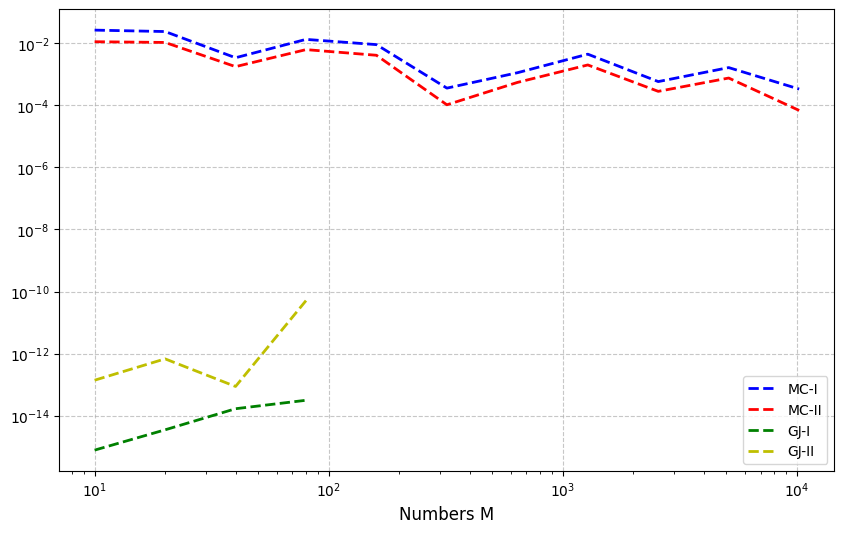
\includegraphics[scale=0.45]{diff_M_err.png}
    \caption{Relative errors of $\btau f(t)$ in Example \ref{eg:1} with different numbers of quadrature points for different numerical integration methods.}
    \label{fig:diff_M_err}
\end{figure}

\paragraph*{\textbf{Various $\alpha$ with sufficient quadrature points}} In this experiment, we investigate the numerical behavior of each method as the fractional order $\alpha$ varies, while maintaining a sufficiently large number of quadrature points to ensure convergence. Specifically, we set $M=10000$ for the Monte Carlo methods and $M=100$ for the Gauss-Jacobi methods. We fix $t=1.5$, $\lambda=-1.0$, and use $\varepsilon=10^{-7}$ for \textbf{MC-I} and \textbf{MC-II}. We assign $\alpha$ values from 100 equidistant nodes within the interval $(1.01, 1.99)$. 

The results, presented in Figure \ref{fig:diff_al}, indicate that as the fractional order $\alpha$ approaches $2$, the accuracy of the Monte Carlo methods deteriorates markedly. This degradation occurs because the probability density function becomes more singular, causing samples to cluster near $0$. Consequently, the introduction of $\varepsilon$ leads to significant discrepancies in Monte Carlo integration, while its omission leads to numerical instabilities. Therefore, the Gauss-Jacobi method emerges as the more robust alternative.   
\begin{figure}[htbp]
    \centering
    \begin{subfigure}{.5\textwidth}
        \centering
        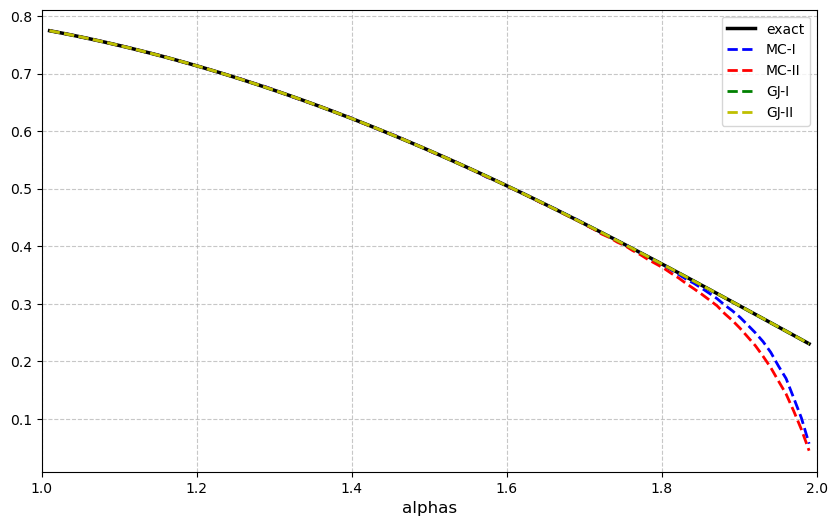
\includegraphics[scale=0.35]{diff_al.png}
        % \caption{$e_{ini,f}$.}
        \end{subfigure}%
        \begin{subfigure}{.5\textwidth}
        \centering
        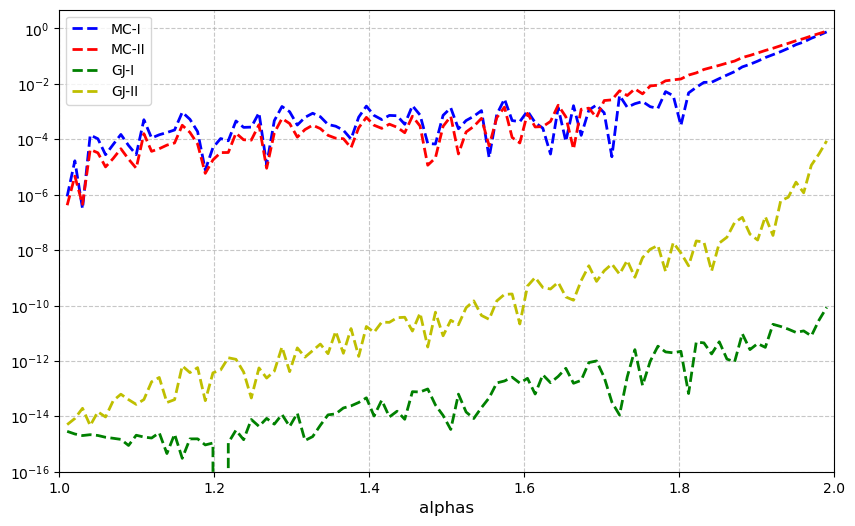
\includegraphics[scale=0.35]{diff_al_error.png}
        % \caption{$e_f^n$ with $t_n=0.5$.}
        \end{subfigure}%
        \caption{Solution profiles of $\btau f(t)$ of Example \ref{eg:1} with different $\al$ for numerical integration methods. Left: the computed $\btau f(t)$ for each method, \textit{exact} means the true $\dta f(t)$. Right: the relative errors $err$ for each method.
        }
    \label{fig:diff_al}
\end{figure}

The numerical results validate the effectiveness of our integrand transformation (\textbf{Type II}). When comparing the Monte Carlo and Gauss-Jacobi approaches, we observe that the Gauss-Jacobi quadratures consistently exhibit superior performance, especially as $\alpha$ approaches $2$. This improvement is primarily attributed to the sensitivity of the Monte Carlo method to the hyperparameter setting of $\varepsilon$, which becomes increasingly critical due to the singular behavior of the integrand near zero in this regime.

The comparison of computational costs is presented in Section \ref{sec:experiments} within the PINNs framework, where we detail the training time required for each numerical integration method. Our proposed tDWfPINNs achieve a substantial reduction in both computation time and GPU resource consumption, indicating a notable gain in computational efficiency. While the Gauss-Jacobi method generally outperforms the Monte Carlo approach, special care must be taken in selecting an appropriate number of quadrature points to balance computational efficiency and approximation accuracy.

\section{Experiments}
\label{sec:experiments}

In this section, we use transformed MCfPINNs in Section \ref{sec:methodology} to solve time-fractional partial differential equations with $\alpha \in (1, 2)$. In the following, we use \textbf{MC-I}, \textbf{MC-II}, \textbf{GJ-I}, and \textbf{GJ-II} to refer to the four numerical integration schemes in Corollary \ref{coro:4}.

To further improve the training performance, we adopt a resampling strategy as described in \cite{Zhang2025}. This approach consists of iterative training cycles, each involving a fixed number of training epochs followed by a resampling of collocation points in the domain. The resampling strategy significantly enhances the convergence behavior of the neural network by mitigating the risk of stagnation in local minima, a common challenge in the training of PINNs. Through this adaptive sampling, the network is better guided toward learning the underlying solution dynamics, particularly in regions with high approximation errors. 

 Unless otherwise specified, we adopt the following settings in all numerical experiments. The neural network architecture consists of 7 hidden layers, each with 20 neurons, and employs the hyperbolic tangent \textit{tanh} as the activation function. This choice ensures that Theorem \ref{thm:represent_2} and Corollary \ref{coro:4} can be applied directly to the smooth neural network solution $u(t,\x;\theta)$. For the Monte Carlo methods, $\varepsilon=10^{-7}$ for \textbf{MC-I} and \textbf{MC-II}. To measure the accuracy of the learned solutions, we use the $L^2$ relative error defined as 
\begin{equation}
    \label{eqn:l2err}
    e_r(\theta) = \frac{\sqrt{\sum_{i=1}^{N} [u(t_i,\x_i;\theta)-u^*(t_i,\x_i)]^2}}{\sqrt{\sum_{i=1}^{N} [u^*(t_i,\x_i)]^2}},
\end{equation}
where $(t_i,\x_i)$, $i=1,2,...,N$ represents the test data set. All training and testing are conducted on an NVIDIA V100 (32 GB).

\subsection{Summary of results and findings}
In this section, we summarize our numerical observations across various problem settings. We present the performance of our proposed methods after training, examine solution behaviors, and explore the limitations of PINNs when applied to time-fractional diffusion-wave equations.

Regarding computational efficiency, our proposed tDWfPINNs significantly reduce both time consumption and GPU resource usage, while preserving a comparable level of accuracy. This makes the transformed numerical scheme highly recommended for solving time-fractional PDEs with orders $\alpha \in (1, 2)$.

Furthermore, the Gauss-Jacobi method typically requires significantly fewer quadrature points than the Monte Carlo method to achieve similar accuracy (as demonstrated in Section \ref{subsec:eg1}). This indicates the potential superiority of the Gauss-Jacobi integration in certain contexts. However, we observe that the wave component introduced by the Mittag-Leffler function can strongly influence the numerical behavior of both the Gauss-Jacobi quadrature and Monte Carlo method. While our experiments consistently favor the Gauss-Jacobi method, its effectiveness is sensitive to the choice of quadrature resolution. Careful tuning of the number of quadrature points is therefore essential to fully exploit its advantages without incurring instability or excessive computational overhead.


\begin{remark}
    We briefly address the stability characteristics of the proposed methods. Our numerical experiments suggest two key observations:
\begin{enumerate}
    \item \textbf{Integration Method:} The Gauss-Jacobi approach consistently exhibits superior stability compared to Monte Carlo integration. This is attributed to the fact that Gauss-Jacobi quadratures are specifically designed to handle the singular weights inherent in fractional operators, whereas Monte Carlo sampling can suffer from high variance near singularities.
    \item \revise{\textbf{Type I vs. Type II:} The transformed formulation (Type II) significantly reduces computational cost by avoiding automatic differentiation at shifted quadrature points. The apparent stronger singularity in Eq. \eqref{eqn:transformed} is removable at the continuous level, and Theorem \ref{thm:stability} shows that Type-I and Type-II have the same representation-level stability bound. The remaining practical sensitivity is therefore a numerical conditioning issue of raw difference quotients and quadrature near $\tau=0$, which is quantified by the regularization-bias estimate in Proposition \ref{prop:regularization-bias}.}
\end{enumerate}
    
\end{remark}

Finally, we conduct numerical experiments on time-fractional Burgers equations with $\alpha \in (1, 2)$ and incorporate the RAD method from \cite{LuLu:2023:RAD}. Unlike the significant improvements RAD provides for integer-order equations, its application in tDWfPINNs yields only marginal improvements. This limited benefit persists even in cases where RAD successfully identifies shock formations in the solution. We hypothesize that this phenomenon stems from the intrinsic wave-like nature of diffusion-wave equations, which introduces complex nonlocal behaviors not present in classical integer-order models. These observations point to the need for further investigation into the interplay between adaptive sampling techniques and the nonlocal memory effects of fractional dynamics.



\subsection{Time-fractional diffusion-wave equations in 1D domain}
\label{subsec:eg1}
In the warm-up stage, we consider the following time-fractional PDEs in $\Omega=(0,1)$ with $\al=1.5$:
\begin{equation}
    \label{eqn:eg1}
    \begin{aligned}
        \dta u(t,x) - u_{xx}(t,x) &= 0,~~ (t,\x)\in (0,1]\times\Omega,\\
        u(t,0)=u(t,1)&=0,~~t\in(0,1],\\
        u(0,x)&=2\sin(\pi x), ~~x\in\Omega,\\
        \partial_tu(0,x)&=-\sin(\pi x), ~~x\in\Omega,
    \end{aligned}
\end{equation}
with the exact solution 
\begin{equation*}
     u(t,x)= (2E_{\al,1}(-\pi^2 t^\al) - t E_{\al,2}(-\pi^2 t^\al))\sin(\pi x)
\end{equation*}
here $E_{\al,\beta}(t)$ is the Mittag-Leffler function (see details in \cite{Podlubny1999,Jin2021:Book}).

The exact solution is depicted in Figure \ref{fig:eg1-exact}. In contrast to (sub)diffusion equations, the solution of the diffusion-wave equation exhibits a distinctive wave-like structure, primarily driven by the Mittag-Leffler functions. This characteristic introduces additional complexity, making such equations potentially more difficult to solve using vanilla PINNs compared to (sub)diffusion equations. To assess the computational performance of the numerical integration methods presented in Corollary \ref{coro:4}, we conducted extensive tests with results summarized in Table \ref{tab:forward}.
\begin{figure}[htbp]
    \centering
    \includegraphics[scale=0.35]{exact-eg1.jpg}
    \caption{Solution profiles of $u(t,x)$ in equation \eqref{eqn:eg1}.}
    \label{fig:eg1-exact}
\end{figure}

For small batches, we sampled 5000 collocation points within the domain, along with 1000 points each on the spatial and temporal boundaries. In the large-batch setting, we increased the sampling density to 10000 points in the domain and 2000 points on both the spatial and temporal boundaries. We set the maximum number of iterations to be $L=10$, with each iteration comprising 5000 epochs trained using the Adam optimizer at a learning rate of $10^{-3}$. The weighting parameter in the loss function \eqref{eqn:loss-forward} was set to 1.0. 

Regarding computational efficiency, our analysis reveals that the transformed schemes exhibit significantly lower and more stable computation times compared to their direct counterparts (\textbf{MC-I} and \textbf{GJ-I}), which demonstrate rapidly increasing computational costs. For each value of $M$ (number of quadrature points), the transformed schemes consistently require substantially less computational time than direct methods; even with $M=16$ for the Gauss-Jacobi method, our proposed method could save several seconds over 5000 epochs. Additionally, the memory usage is markedly reduced. For instance, with small batches at $M=1280$, \textbf{MC-II} consumes only 10.5GB of GPU memory, whereas \textbf{MC-I} requires 29.1GB. This reduced memory footprint enables the transformed MCfPINNs to accommodate denser sampling points and larger $M$ within a single GPU environment. Importantly, these gains in efficiency come without sacrificing numerical accuracy; both integration types maintain comparable error levels.

Moreover, the Gauss-Jacobi quadrature method appears to offer computational advantages over the Monte Carlo approach, as it requires fewer quadrature points to achieve comparable levels of accuracy, further reinforcing its suitability for efficient and precise fractional-order computations.

\begin{table}[htbp]

    \centering
    \begin{tabular}{|c|cc|cc|c|cc|cc|}
        \hline
        Cases    & \multicolumn{2}{c|}{Small batches}                                                                                                        & \multicolumn{2}{c|}{Large batches}                                                                                                       &          & \multicolumn{2}{c|}{Small batches}                                                                                                     & \multicolumn{2}{c|}{Large batches}                                                                                                     \\ \hline
        $M$/Type & \multicolumn{1}{c|}{\textbf{MC-I}}                                             & \textbf{MC-II}                                           & \multicolumn{1}{c|}{\textbf{MC-I}}                                            & \textbf{MC-II}                                           & $M$/Type & \multicolumn{1}{c|}{\textbf{GJ-I}}                                           & \textbf{GJ-II}                                          & \multicolumn{1}{c|}{\textbf{GJ-I}}                                           & \textbf{GJ-II}                                          \\ \hline
        $M=80$   & \multicolumn{1}{c|}{\begin{tabular}[c]{@{}c@{}}1.91e-1\\ 5m26s\end{tabular}}   & \begin{tabular}[c]{@{}c@{}}8.87e-2\\ 4m03s\end{tabular}  & \multicolumn{1}{c|}{\begin{tabular}[c]{@{}c@{}}1.12e-1\\ 8m55s\end{tabular}}  & \begin{tabular}[c]{@{}c@{}}6.16e-2\\ 5m22s\end{tabular}  & $M=16$   & \multicolumn{1}{c|}{\begin{tabular}[c]{@{}c@{}}7.74e-2\\ 2m57s\end{tabular}} & \begin{tabular}[c]{@{}c@{}}6.31e-2\\ 2m57s\end{tabular} & \multicolumn{1}{c|}{\begin{tabular}[c]{@{}c@{}}4.38e-2\\ 3m37s\end{tabular}} & \begin{tabular}[c]{@{}c@{}}3.80e-2\\ 3m19s\end{tabular} \\ \hline
        $M=160$  & \multicolumn{1}{c|}{\begin{tabular}[c]{@{}c@{}}1.10e-1\\ 8m51s\end{tabular}}   & \begin{tabular}[c]{@{}c@{}}5.76e-2\\ 5m17s\end{tabular}  & \multicolumn{1}{c|}{\begin{tabular}[c]{@{}c@{}}1.09e-1\\ 15m34s\end{tabular}} & \begin{tabular}[c]{@{}c@{}}8.61e-2\\ 8m38s\end{tabular}  & $M=32$   & \multicolumn{1}{c|}{\begin{tabular}[c]{@{}c@{}}3.92e-2\\ 3m24s\end{tabular}} & \begin{tabular}[c]{@{}c@{}}2.93e-2\\ 3m01s\end{tabular} & \multicolumn{1}{c|}{\begin{tabular}[c]{@{}c@{}}3.93e-2\\ 5m06s\end{tabular}} & \begin{tabular}[c]{@{}c@{}}3.28e-2\\ 3m39s\end{tabular} \\ \hline
        $M=320$  & \multicolumn{1}{c|}{\begin{tabular}[c]{@{}c@{}}8.20e-2\\ 15 m33s\end{tabular}} & \begin{tabular}[c]{@{}c@{}}4.11e-2\\ 8m34s\end{tabular}  & \multicolumn{1}{c|}{\begin{tabular}[c]{@{}c@{}}9.67e-2\\ 24m02s\end{tabular}} & \begin{tabular}[c]{@{}c@{}}4.44e-2\\ 10m52s\end{tabular} & $M=48$   & \multicolumn{1}{c|}{\begin{tabular}[c]{@{}c@{}}3.05e-2\\ 4m12s\end{tabular}} & \begin{tabular}[c]{@{}c@{}}4.83e-2\\ 3m21s\end{tabular} & \multicolumn{1}{c|}{\begin{tabular}[c]{@{}c@{}}4.82e-2\\ 6m19s\end{tabular}} & \begin{tabular}[c]{@{}c@{}}6.01e-2\\ 4m13s\end{tabular} \\ \hline
        $M=640$  & \multicolumn{1}{c|}{\begin{tabular}[c]{@{}c@{}}1.05e-1\\ 24m04s\end{tabular}}  & \begin{tabular}[c]{@{}c@{}}7.65e-2\\ 10m40s\end{tabular} & \multicolumn{1}{c|}{\begin{tabular}[c]{@{}c@{}}7.94e-2\\ 45m10s\end{tabular}} & \begin{tabular}[c]{@{}c@{}}5.54e-2\\ 19m45s\end{tabular} & $M=64$   & \multicolumn{1}{c|}{\begin{tabular}[c]{@{}c@{}}4.87e-2\\ 5m02s\end{tabular}} & \begin{tabular}[c]{@{}c@{}}4.46e-2\\ 3m34s\end{tabular} & \multicolumn{1}{c|}{\begin{tabular}[c]{@{}c@{}}3.21e-2\\ 7m38s\end{tabular}} & \begin{tabular}[c]{@{}c@{}}3.78e-2\\ 4m35s\end{tabular} \\ \hline
        $M=1280$ & \multicolumn{1}{c|}{\begin{tabular}[c]{@{}c@{}}7.0e-2\\ 45m10s\end{tabular}}   & \begin{tabular}[c]{@{}c@{}}5.82e-2\\ 19m44s\end{tabular} & \multicolumn{1}{c|}{OoM}                                                      & \begin{tabular}[c]{@{}c@{}}5.64e-2\\ 37m25s\end{tabular} & $M=80$   & \multicolumn{1}{c|}{\begin{tabular}[c]{@{}c@{}}6.29e-2\\ 5m27s\end{tabular}} & \begin{tabular}[c]{@{}c@{}}6.73e-2\\ 3m56s\end{tabular} & \multicolumn{1}{c|}{\begin{tabular}[c]{@{}c@{}}5.35e-2\\ 8m50s\end{tabular}} & \begin{tabular}[c]{@{}c@{}}3.66e-2\\ 5m17s\end{tabular} \\ \hline
        \end{tabular}

    \caption{$L^2$ relative error and computational time for equation \eqref{eqn:eg1} with different $M$ and number of points. For each grid, the first row is the relative error, the second row is the average computational time for 5000 epochs. OoM means out of memory.}
    \label{tab:forward}
\end{table}

In the following, we present solution profiles derived from the results in Table \ref{tab:forward}. We first compare the cases of the Monte Carlo method in Figure \ref{fig:eg1sol}, which displays the solution profiles and absolute errors for each numerical method.  The results indicate that improved accuracy in the computation of fractional derivatives leads to more effective training outcomes. At relatively low values of $M$, the Monte Carlo methods suffer from reduced accuracy, emphasizing the advantage of Gauss-Jacobi methods in achieving better performance with fewer quadrature points. This highlights the superior computational efficiency of Gauss-Jacobi quadratures in practice.
\begin{figure}[htbp]
    \centering
    \begin{subfigure}{.25\textwidth}
        \centering
        \includegraphics[height=0.75\textwidth,width=1.0\textwidth]{solution-EG1-small-batch-seed229-MC-I_80.jpg}
    \end{subfigure}%
    \begin{subfigure}{.25\textwidth}
        \centering
        \includegraphics[height=0.75\textwidth,width=1.0\textwidth]{solution-EG1-small-batch-seed229-MC-II_80.jpg}
    \end{subfigure}%
    \begin{subfigure}{.25\textwidth}
        \centering
        \includegraphics[height=0.75\textwidth,width=1.0\textwidth]{solution-EG1-small-batch-seed229-MC-I_640.jpg}
    \end{subfigure}%
    \begin{subfigure}{.25\textwidth}
        \centering
        \includegraphics[height=0.75\textwidth,width=1.0\textwidth]{solution-EG1-small-batch-seed229-MC-II_640.jpg}
    \end{subfigure}%
    \newline
    \raggedleft
    \begin{subfigure}{.25\textwidth}
        \centering
        \includegraphics[height=0.75\textwidth,width=1.0\textwidth]{error-EG1-small-batch-seed229-MC-I_80.jpg}
        \caption{\textbf{MC-I}, $M=80$.}
    \end{subfigure}%
    \begin{subfigure}{.25\textwidth}
        \centering
        \includegraphics[height=0.75\textwidth,width=1.0\textwidth]{error-EG1-small-batch-seed229-MC-II_80.jpg}
        \caption{\textbf{MC-II}, $M=80$.}
    \end{subfigure}%
    \begin{subfigure}{.25\textwidth}
        \centering
        \includegraphics[height=0.75\textwidth,width=1.0\textwidth]{error-EG1-small-batch-seed229-MC-I_640.jpg}
        \caption{\textbf{MC-I}, $M=640$.}
    \end{subfigure}%
    \begin{subfigure}{.25\textwidth}
        \centering
        \includegraphics[height=0.75\textwidth,width=1.0\textwidth]{error-EG1-small-batch-seed229-MC-II_640.jpg}
        \caption{\textbf{MC-II}, $M=640$.}
    \end{subfigure}%
    \caption{Profiles of absolute error and neural network solutions for equation \eqref{eqn:eg1} with the Monte Carlo method for $M=80$ and $M=640$. First row: numerical solutions. Second row: absolute error.}
    \label{fig:eg1sol}
\end{figure}

However, the Gauss-Jacobi quadrature method demonstrates remarkable efficiency in terms of the number of quadrature points required. As illustrated in Figure \ref{fig:eg1sol640}, which compares solution profiles and absolute error distributions for implementations with $M=16$ and $M=80$, the method achieves comparable accuracy levels with significantly fewer quadrature points. 

\begin{figure}[htbp]
    \centering
    \begin{subfigure}{.25\textwidth}
        \centering
        \includegraphics[height=0.75\textwidth,width=1.0\textwidth]{solution-EG1-small-batch-seed229-GJ-I_16.jpg}
    \end{subfigure}%
    \begin{subfigure}{.25\textwidth}
        \centering
        \includegraphics[height=0.75\textwidth,width=1.0\textwidth]{solution-EG1-small-batch-seed229-GJ-II_16.jpg}
    \end{subfigure}%
    \begin{subfigure}{.25\textwidth}
        \centering
        \includegraphics[height=0.75\textwidth,width=1.0\textwidth]{solution-EG1-small-batch-seed229-GJ-I_80.jpg}
    \end{subfigure}%
    \begin{subfigure}{.25\textwidth}
        \centering
        \includegraphics[height=0.75\textwidth,width=1.0\textwidth]{solution-EG1-small-batch-seed229-GJ-II_80.jpg}
    \end{subfigure}%
    \newline
    \raggedleft
    \begin{subfigure}{.25\textwidth}
        \centering
        \includegraphics[height=0.75\textwidth,width=1.0\textwidth]{error-EG1-small-batch-seed229-GJ-I_16.jpg}
        \caption{\textbf{GJ-I}, $M=16$.}
    \end{subfigure}%
    \begin{subfigure}{.25\textwidth}
        \centering
        \includegraphics[height=0.75\textwidth,width=1.0\textwidth]{error-EG1-small-batch-seed229-GJ-II_16.jpg}
        \caption{\textbf{GJ-II}, $M=16$.}
    \end{subfigure}%
    \begin{subfigure}{.25\textwidth}
        \centering
        \includegraphics[height=0.75\textwidth,width=1.0\textwidth]{error-EG1-small-batch-seed229-GJ-I_80.jpg}
        \caption{\textbf{GJ-I}, $M=80$.}
    \end{subfigure}%
    \begin{subfigure}{.25\textwidth}
        \centering
        \includegraphics[height=0.75\textwidth,width=1.0\textwidth]{error-EG1-small-batch-seed229-GJ-II_80.jpg}
        \caption{\textbf{GJ-II}, $M=80$.}
    \end{subfigure}%
    \caption{Profiles of absolute error and neural network solutions for equation \eqref{eqn:eg1} with the Gauss-Jacobi method for $M=16$ and $M=80$. First row: numerical solutions. Second row: absolute error.}
    \label{fig:eg1sol640}
\end{figure}



\subsection{Time-fractional Diffusion-Wave equation with adjusted parameters}
\label{subsec:eg2}
Here we consider the following time-fractional PDEs in $\Omega=(0,1)$:
\begin{equation}
    \label{eqn:eg2}
    \begin{aligned}
        \dta u(t,x) - \frac{\lambda }{k^2\pi^2} u_{xx}(t,x) &= 0,~~ (t,\x)\in (0,T]\times\Omega, ~~\lambda\in\mathbb{R}^+,~~ k\in\mathbb{N}, \\
        u(t,0)=u(t,1)&=0,~~t\in(0,T],\\
        u(0,x)&=\sin(k\pi x), ~~x\in\Omega,\\
        \partial_tu(0,x)&=-0.5\sin(k\pi x), ~~x\in\Omega,
    \end{aligned}
\end{equation}
with  exact solution 
\begin{equation*}
    u(t,x)=  (E_{\al, 1}(-\lambda t^\al)-0.5tE_{\al,2}(-\lambda t^\al))\sin(k\pi x).
\end{equation*}

Equation \eqref{eqn:eg1} can be regarded as a special case with $\lambda = \pi^2$, $k=1$, scaled initial conditions, and $T=1$. In Table \ref{tab:eg2-1}, the final time is set to $T=2$. Small batches, consistent with those in subsection \ref{subsec:eg1}, are adopted. The training procedure is configured with a maximum of  $L=3$ iterations, each consisting of 5000 epochs and optimized using the Adam optimizer with a learning rate of  $0.001$. The exact solutions for each case and each $\alpha$ are presented in Figure \ref{fig:eg2-exact}, allowing a clear comparison of the diffusion and wave components in the solutions. As $\alpha$ increases, the wave component becomes more pronounced, while larger values of the diffusion coefficient $\lambda/(k^2\pi^2)$ enhance the influence of the diffusion effects. This interplay between the wave and diffusion components helps explain the numerical behaviors observed in the subsequent results.
\begin{figure}[htbp]
    \centering
    \begin{subfigure}{.25\textwidth}
        \centering
        \includegraphics[height=0.75\textwidth,width=1.0\textwidth]{exact-125-k1lam1.jpg}
    \end{subfigure}%
    \begin{subfigure}{.25\textwidth}
        \centering
        \includegraphics[height=0.75\textwidth,width=1.0\textwidth]{exact-125-k2lam4.jpg}
    \end{subfigure}%
    \begin{subfigure}{.25\textwidth}
        \centering
        \includegraphics[height=0.75\textwidth,width=1.0\textwidth]{exact-125-k4lam4.jpg}
    \end{subfigure}%
    \begin{subfigure}{.25\textwidth}
        \centering
        \includegraphics[height=0.75\textwidth,width=1.0\textwidth]{exact-125-k6lam6.jpg}
    \end{subfigure}%
    \newline
    \raggedleft
    \begin{subfigure}{.25\textwidth}
        \centering
        \includegraphics[height=0.75\textwidth,width=1.0\textwidth]{exact-150-k1lam1.jpg}
    \end{subfigure}%
    \begin{subfigure}{.25\textwidth}
        \centering
        \includegraphics[height=0.75\textwidth,width=1.0\textwidth]{exact-150-k2lam4.jpg}
    \end{subfigure}%
    \begin{subfigure}{.25\textwidth}
        \centering
        \includegraphics[height=0.75\textwidth,width=1.0\textwidth]{exact-150-k4lam4.jpg}
    \end{subfigure}%
    \begin{subfigure}{.25\textwidth}
        \centering
        \includegraphics[height=0.75\textwidth,width=1.0\textwidth]{exact-150-k6lam6.jpg}
    \end{subfigure}%
    \newline
    \raggedleft
    \begin{subfigure}{.25\textwidth}
        \centering
        \includegraphics[height=0.75\textwidth,width=1.0\textwidth]{exact-175-k1lam1.jpg}
        \caption{\textbf{$k=1$, $\lambda=1$}}
    \end{subfigure}%
    \begin{subfigure}{.25\textwidth}
        \centering
        \includegraphics[height=0.75\textwidth,width=1.0\textwidth]{exact-175-k2lam4.jpg}
        \caption{$k=2$, $\lambda=4$}
    \end{subfigure}%
    \begin{subfigure}{.25\textwidth}
        \centering
        \includegraphics[height=0.75\textwidth,width=1.0\textwidth]{exact-175-k4lam4.jpg}
        \caption{$k=4$, $\lambda=4$}
    \end{subfigure}%
    \begin{subfigure}{.25\textwidth}
        \centering
        \includegraphics[height=0.75\textwidth,width=1.0\textwidth]{exact-175-k6lam6.jpg}
        \caption{$k=6$, $\lambda=6$}
    \end{subfigure}%
    \caption{Exact solution of cases in Table \ref{tab:eg2-1} with different $\alpha$, $k$ and $\lambda$. In the first row, $\alpha=1.25$, in the second row, $\alpha=1.5$, in the third row, $\alpha=1.75$.}
    \label{fig:eg2-exact}
\end{figure}

We present the relative errors and computational time in Table \ref{tab:eg2-1} for different numerical integration schemes and values of $M$. The proposed tDWfPINNs demonstrate accuracy on par with direct numerical integration methods, while significantly reducing computational time. These extensive numerical experiments further validate the efficiency of our approach in solving the time-fractional diffusion-wave equation.
% \usepackage{tabularray}
\begin{table}
\centering

\begin{tblr}{
  cells = {c},
  cell{1}{3} = {c=2}{},
  cell{1}{5} = {c=2}{},
  cell{1}{8} = {c=2}{},
  cell{1}{10} = {c=2}{},
  cell{3}{1} = {r=2}{},
  cell{5}{1} = {r=2}{},
  cell{7}{1} = {r=2}{},
  cell{9}{3} = {c=2}{},
  cell{9}{5} = {c=2}{},
  cell{9}{8} = {c=2}{},
  cell{9}{10} = {c=2}{},
  cell{10}{1} = {r=2}{},
  cell{12}{1} = {r=2}{},
  cell{14}{1} = {r=2}{},
  vlines,
  hline{1-3,5,7,9-10,12,14,16} = {-}{},
  hline{4,6,8,11,13,15} = {2-11}{},
}
         &         & $k=1$, $\lambda=1$ &                    & $k=2$, $\lambda=4$ &                    &        & $k=1$, $\lambda=1$  &                   & $k=2$, $\lambda=4$ &                   \\
$\alpha$ &         & \textbf{MC-I}      & \textbf{MC-II}     & \textbf{MC-I}      & \textbf{MC-II}     &        & \textbf{GJ-I}       & \textbf{GJ-II}    & \textbf{GJ-I}      & \textbf{GJ-II}    \\
$1.25$   & $M=80$  & {2.16e-2\\ 5m38s}  & {3.15e-2\\ 4m04s}  & {4.58e-2\\ 5m39s}  & {4.63e-2\\ 3m59s}  & $M=16$ & {5.80e-3\\ 3m13s}   & {1.03e-2\\ 2m51s} & {4.74e-2\\ 3m11s}  & {7.06e-2\\ 3m01s} \\
         & $M=640$ & {1.93e-2\\ 24m00s} & {1.10e-2\\ 10m52s} & {6.75e-2\\ 23m57s} & {3.76e-2\\ 10m53s} & $M=80$ & {7.10e-3\\ 5m31s}   & {7.60e-3\\ 4m01s} & {6.32e-2\\ 5m35s}  & {3.96e-2\\ 3m51s} \\
$1.5$    & $M=80$  & {3.83e-2\\ 5m36s}  & {8.50e-3\\ 4m06s}  & {6.51e-2\\ 5m36s}  & {4.75e-2\\ 3m52s}  & $M=16$ & {1.20e-2\\ 3m08s}   & {1.14e-2\\ 2m59s} & {3.24e-2\\ 3m07s}  & {4.21e-2\\ 3m01s} \\
         & $M=640$ & {4.35e-2\\ 23m55s} & {2.35e-2\\ 10m49s} & {5.13e-2\\ 23m56s} & {2.48e-2\\ 10m53s} & $M=80$ & {6.10e-3\\ 5m31s}   & {1.82e-2\\ 4m04s} & {2.74e-2\\ 5m31s}  & {2.20e-2\\ 3m53s} \\
$1.75$   & $M=80$  & {7.20e-3\\ 5m32s}  & {7.10e-3\\ 4m05s}  & {6.39e-2\\ 5m34s}  & {2.59e-2\\ 3m54s}  & $M=16$ & {4.1e-3\\ 3m15s}    & {2.40e-3\\ 3m00s} & {1.64e-2\\ 3m07s}  & {2.00e-2\\ 2m59s} \\
         & $M=640$ & {4.50e-3\\ 24m02s} & {1.74e-2\\ 10m52s} & {2.64e-2\\ 23m58s} & {2.49e-2\\ 10m52s} & $M=80$ & {1.19e-2\\ 5m32s}   & {8.90e-3\\ 4m00s} & {1.82e-2\\ 5m31s}  & {9.30e-3\\ 3m55s} \\
         &         & $k=4$, $\lambda=4$ &                    & $k=6$, $\lambda=6$ &                    &        & $k=4$, $\lambda =4$ &                   & $k=6$, $\lambda=6$ &                   \\
$1.25$   & $M=80$  & {5.69e-2\\ 5m39s}  & {3.91e-2\\ 3m59s}  & {1.52e-1\\ 5m39s}  & {2.98e-1\\ 3m54s}  & $M=16$ & {6.34e-2\\ 3m07s}   & {6.23e-2\\ 2m59s} & {1.09e-1\\ 3m03s}  & {9.56e-2\\ 3m00s} \\
         & $M=640$ & {2.76e-2\\ 23m59s} & {5.13e-2\\ 10m47s} & {1.01e-1\\ 23m53s} & {1.22e-1\\ 10m52s} & $M=80$ & {3.80e-2\\ 5m36s}   & {5.22e-2\\ 4m01s} & {1.04e-1\\ 5m31s}  & {1.20e-1\\ 4m01s}  \\
$1.5$    & $M=80$  & {4.64e-2\\ 5m41s}  & {3.94e-2\\ 4m06s}  & {6.41e-2\\ 5m33s}  & {5.68e-2\\ 4m10s}  & $M=16$ & {3.60e-2\\ 3m07s}   & {3.96e-2\\ 3m00s} & {4.69e-2\\ 3m05s}  & {5.41e-2\\ 2m56s} \\
         & $M=640$ & {4.65e-2\\ 23m52s} & {6.76e-2\\ 10m52s} & {8.74e-2\\ 23m54s} & {5.28e-2\\ 10m54s} & $M=80$ & {2.84e-2\\ 5m33s}   & {2.25e-2\\ 3m58s} & {4.29e-2\\ 5m39s}  & {8.75e-2\\ 4m07s} \\
$1.75$   & $M=80$  & {9.74e-2\\ 5m35s}  & {3.78e-2\\ 3m55s}  & {6.10e-2\\ 5m42s}  & {8.12e-2\\ 4m05s}  & $M=16$ & {7.48e-2\\3m07s}    & {3.37e-2\\3m02s}  & {5.45e-2\\ 3m05s}  & {3.44e-2\\2m59s}  \\
         & $M=640$ & {2.59e-2\\ 23m58s} & {3.88e-2\\ 10m51s} & {5.28e-2\\ 23m55s} & {6.71e-2\\ 10m52s} & $M=80$ & {3.62e-2\\ 5m31s}   & {5.13e-2\\ 3m54s} & {4.76e-2\\ 5m30s}  & {1.99e-2\\ 4m04s} 
\end{tblr}
\caption{Results of different numerical integrations with different parameters in equation \eqref{eqn:eg2}. In each grid, the first row is the $L^2$ relative error, the second row is the computational time for each case within 5000 epochs.}
\label{tab:eg2-1}
\end{table}

As the training process for PINNs progresses, our experiments consistently demonstrate that the Gauss-Jacobi method outperforms the Monte Carlo approach. However, we observe that the performance of both methods tends to deteriorate as the equation parameter increases, implying an increase in solution complexity.

Examining Table \ref{tab:eg2-1}, we observe that for cases involving larger values of $\lambda$ and $k$, models with higher fractional order $\alpha$ tend to produce more accurate results than those with smaller $\alpha$. This trend is likely attributable to the strong decay in the Mittag-Leffler scaling factor for small $\alpha$ when $\lambda$ is large, as demonstrated in Figure \ref{fig:eg2-exact}.

To further elucidate this behavior, Figure \ref{fig:eg2-err-1} presents the absolute error distributions of \textbf{MC-II} and \textbf{GJ-II} for cases with $k=2, \lambda=4$ and $k=4, \lambda=4$, evaluated across various $\alpha$ values when $M=640$ and $M=80$. The error patterns revealed in this figure lead to two significant observations. First, the error patterns obtained using the Gauss-Jacobi method tend to exhibit higher frequency content than those from the Monte Carlo method. This is indicative of a more effective representation of the underlying solution features and aligns with theoretical insights derived from neural tangent kernel analysis, such as those presented in \cite{WangYuParis:2022:NTK}. Second, significant error concentrations are consistently observed near the initial temporal layer and spatial boundaries. This suggests that the design of future training strategies—such as boundary-focused sampling or adaptive loss weighting—should prioritize these regions to improve overall approximation quality.

\begin{figure}[htbp]
    \centering
    \begin{subfigure}{.25\textwidth}
        \centering
        \includegraphics[height=0.75\textwidth,width=1.0\textwidth]{error-DW-table-seed229-MC-II_M640_AL1.25_k2_lam4.jpg}
    \end{subfigure}%
    \begin{subfigure}{.25\textwidth}
        \centering
        \includegraphics[height=0.75\textwidth,width=1.0\textwidth]{error-DW-table-seed229-GJ-II_M80_AL1.25_k2_lam4.jpg}
    \end{subfigure}%
    \begin{subfigure}{.25\textwidth}
        \centering
        \includegraphics[height=0.75\textwidth,width=1.0\textwidth]{error-DW-table-seed229-MC-II_M640_AL1.25_k4_lam4.jpg}
    \end{subfigure}%
    \begin{subfigure}{.25\textwidth}
        \centering
        \includegraphics[height=0.75\textwidth,width=1.0\textwidth]{error-DW-table-seed229-GJ-II_M80_AL1.25_k4_lam4.jpg}
    \end{subfigure}%
    \newline
    \raggedleft
    \begin{subfigure}{.25\textwidth}
        \centering
        \includegraphics[height=0.75\textwidth,width=1.0\textwidth]{error-DW-table-seed229-MC-II_M640_AL1.50_k2_lam4.jpg}
    \end{subfigure}%
    \begin{subfigure}{.25\textwidth}
        \centering
        \includegraphics[height=0.75\textwidth,width=1.0\textwidth]{error-DW-table-seed229-GJ-II_M80_AL1.50_k2_lam4.jpg}
    \end{subfigure}%
    \begin{subfigure}{.25\textwidth}
        \centering
        \includegraphics[height=0.75\textwidth,width=1.0\textwidth]{error-DW-table-seed229-MC-II_M640_AL1.50_k4_lam4.jpg}
    \end{subfigure}%
    \begin{subfigure}{.25\textwidth}
        \centering
        \includegraphics[height=0.75\textwidth,width=1.0\textwidth]{error-DW-table-seed229-GJ-II_M80_AL1.50_k4_lam4.jpg}
    \end{subfigure}%
    \newline
    \raggedleft
    \begin{subfigure}{.25\textwidth}
        \centering
        \includegraphics[height=0.75\textwidth,width=1.0\textwidth]{error-DW-table-seed229-MC-II_M640_AL1.75_k2_lam4.jpg}
        \caption{\textbf{MC-II}, $k=2$, $\lambda=4$, $M=640$.}
    \end{subfigure}%
    \begin{subfigure}{.25\textwidth}
        \centering
        \includegraphics[height=0.75\textwidth,width=1.0\textwidth]{error-DW-table-seed229-GJ-II_M80_AL1.75_k2_lam4.jpg}
        \caption{\textbf{GJ-II}, $k=2$, $\lambda=4$, $M=80$.}
    \end{subfigure}%
    \begin{subfigure}{.25\textwidth}
        \centering
        \includegraphics[height=0.75\textwidth,width=1.0\textwidth]{error-DW-table-seed229-MC-II_M640_AL1.75_k4_lam4.jpg}
        \caption{\textbf{MC-II}, $k=4$, $\lambda=4$, $M=640$.}
    \end{subfigure}%
    \begin{subfigure}{.25\textwidth}
        \centering
        \includegraphics[height=0.75\textwidth,width=1.0\textwidth]{error-DW-table-seed229-GJ-II_M80_AL1.75_k4_lam4.jpg}
        \caption{\textbf{GJ-II}, $k=4$, $\lambda=4$, $M=80$.}
    \end{subfigure}%
    \caption{Absolute errors of cases in Table \ref{tab:eg2-1} with different $\alpha$, $k$ and $\lambda$. In the first row, $\alpha=1.25$, in the second row, $\alpha=1.5$, in the third row, $\alpha=1.75$.}
    \label{fig:eg2-err-1}
\end{figure}

In the following experiments, the number $M$ is fixed at 80, and we employ the transformed schemes exclusively. This choice is motivated by earlier findings demonstrating that the transformed methods attain comparable accuracy to their direct counterparts while significantly reducing computational overhead.

To further investigate the observed performance discrepancies among different configurations, we conducted extended training experiments with sufficient iterations. Specifically, for the cases presented in Table \ref{tab:eg2-1}, comprehensive training was implemented using the Adam optimizer with a learning rate of $10^{-5}$ and $L=50$. The corresponding numerical outcomes are documented in Table \ref{tab:largeL}. With sufficient training, both methods demonstrate enhanced solution accuracy when $\lambda$ is relatively small; however, as $\lambda$ increases, performance degradation becomes evident, highlighting the influence of the diffusion component on solution scaling. The Gauss-Jacobi method consistently outperforms the Monte Carlo approach under these extended training conditions. This suggests that for smaller M, the Monte Carlo integration lacks sufficient resolution to capture solution features effectively, leading to suboptimal training convergence. Consequently, when employing Monte Carlo-based integration within PINNs, a significantly larger number of quadrature samples is advisable to ensure acceptable accuracy. Figure \ref{fig:err-largeL} illustrates the absolute errors, revealing that the error patterns of \textbf{GJ-II} continue to present the high-frequency error structure, implying the better resolution of the Gauss-Jacobi method. 
\begin{table}[htbp]
    \centering
    
    \begin{tabular}{|c|cc|cc|}
        \hline
                      & \multicolumn{2}{c|}{$k=1$, $\lambda=1$}                & \multicolumn{2}{c|}{$k=2$, $\lambda=4$}              \\ \hline
                      & \multicolumn{1}{c|}{\textbf{MC-II}}  & \textbf{GJ-II}  & \multicolumn{1}{c|}{\textbf{MC-II}} & \textbf{GJ-II} \\ \hline
        $\alpha=1.25$ & \multicolumn{1}{c|}{3.30e-3}          & 2.70e-3      & \multicolumn{1}{c|}{3.76e-2}        & 3.12e-2        \\ \hline
        $\alpha=1.5$ & \multicolumn{1}{c|}{3.20e-3}          & 1.60e-3         & \multicolumn{1}{c|}{2.65e-2}        & 1.66e-2        \\ \hline
        $\alpha=1.75$ & \multicolumn{1}{c|}{4.20e-3}          & 9.00e-4         & \multicolumn{1}{c|}{2.85e-2}        & 8.40e-3        \\ \hline
                      & \multicolumn{2}{c|}{$k=4$, $\lambda=4$} & \multicolumn{2}{c|}{$k=6$, $\lambda=6$}              \\ \hline
        $\alpha=1.25$ & \multicolumn{1}{c|}{2.07e-2}         & 2.01e-2         & \multicolumn{1}{c|}{8.82e-2}        & 5.96e-2        \\ \hline
        $\alpha=1.5$ & \multicolumn{1}{c|}{1.67e-2}          & 1.39e-2         & \multicolumn{1}{c|}{2.37e-2}        & 2.17e-2        \\ \hline
        $\alpha=1.75$ & \multicolumn{1}{c|}{2.60e-2}         & 1.16e-2        & \multicolumn{1}{c|}{6.47e-2}        & 1.58e-2        \\ \hline
        \end{tabular}
    \caption{Relative errors under sufficient training with $L=50$ and learning rate $10^{-5}$.}
    \label{tab:largeL}
    \end{table}
    \begin{figure}[htbp]
        \centering
        \begin{subfigure}{.25\textwidth}
            \centering
            \includegraphics[height=0.75\textwidth,width=1.0\textwidth]{error-DW-sufficient-seed229-MC-II_M80_AL1.25_k1_lam1.jpg}
        \end{subfigure}%
        \begin{subfigure}{.25\textwidth}
            \centering
            \includegraphics[height=0.75\textwidth,width=1.0\textwidth]{error-DW-sufficient-seed229-GJ-II_M80_AL1.25_k1_lam1.jpg}
        \end{subfigure}%
        \begin{subfigure}{.25\textwidth}
            \centering
            \includegraphics[height=0.75\textwidth,width=1.0\textwidth]{error-DW-sufficient-seed229-MC-II_M80_AL1.25_k2_lam4.jpg}
        \end{subfigure}%
        \begin{subfigure}{.25\textwidth}
            \centering
            \includegraphics[height=0.75\textwidth,width=1.0\textwidth]{error-DW-sufficient-seed229-GJ-II_M80_AL1.25_k2_lam4.jpg}
        \end{subfigure}%
        \newline
        \raggedleft
        \begin{subfigure}{.25\textwidth}
            \centering
            \includegraphics[height=0.75\textwidth,width=1.0\textwidth]{error-DW-sufficient-seed229-MC-II_M80_AL1.50_k1_lam1.jpg}
        \end{subfigure}%
        \begin{subfigure}{.25\textwidth}
            \centering
            \includegraphics[height=0.75\textwidth,width=1.0\textwidth]{error-DW-sufficient-seed229-GJ-II_M80_AL1.50_k1_lam1.jpg}
        \end{subfigure}%
        \begin{subfigure}{.25\textwidth}
            \centering
            \includegraphics[height=0.75\textwidth,width=1.0\textwidth]{error-DW-sufficient-seed229-MC-II_M80_AL1.50_k2_lam4.jpg}
        \end{subfigure}%
        \begin{subfigure}{.25\textwidth}
            \centering
            \includegraphics[height=0.75\textwidth,width=1.0\textwidth]{error-DW-sufficient-seed229-GJ-II_M80_AL1.50_k2_lam4.jpg}
        \end{subfigure}%
        \newline
        \raggedleft
        \begin{subfigure}{.25\textwidth}
            \centering
            \includegraphics[height=0.75\textwidth,width=1.0\textwidth]{error-DW-sufficient-seed229-MC-II_M80_AL1.75_k1_lam1.jpg}
            \caption{\textbf{MC-II}, $k=1$, $\lambda=1$.}
        \end{subfigure}%
        \begin{subfigure}{.25\textwidth}
            \centering
            \includegraphics[height=0.75\textwidth,width=1.0\textwidth]{error-DW-sufficient-seed229-GJ-II_M80_AL1.75_k1_lam1.jpg}
            \caption{\textbf{GJ-II}, $k=1$, $\lambda=1$.}
        \end{subfigure}%
        \begin{subfigure}{.25\textwidth}
            \centering
            \includegraphics[height=0.75\textwidth,width=1.0\textwidth]{error-DW-sufficient-seed229-MC-II_M80_AL1.75_k2_lam4.jpg}
            \caption{\textbf{MC-II}, $k=2$, $\lambda=4$.}
        \end{subfigure}%
        \begin{subfigure}{.25\textwidth}
            \centering
            \includegraphics[height=0.75\textwidth,width=1.0\textwidth]{error-DW-sufficient-seed229-GJ-II_M80_AL1.75_k2_lam4.jpg}
            \caption{\textbf{GJ-II}, $k=2$, $\lambda=4$.}
        \end{subfigure}%
        \newline
        \raggedleft
        \begin{subfigure}{.25\textwidth}
            \centering
            \includegraphics[height=0.75\textwidth,width=1.0\textwidth]{error-DW-sufficient-seed229-MC-II_M80_AL1.25_k4_lam4.jpg}
        \end{subfigure}%
        \begin{subfigure}{.25\textwidth}
            \centering
            \includegraphics[height=0.75\textwidth,width=1.0\textwidth]{error-DW-sufficient-seed229-GJ-II_M80_AL1.25_k4_lam4.jpg}
        \end{subfigure}%
        \begin{subfigure}{.25\textwidth}
            \centering
            \includegraphics[height=0.75\textwidth,width=1.0\textwidth]{error-DW-sufficient-seed229-MC-II_M80_AL1.25_k6_lam6.jpg}
        \end{subfigure}%
        \begin{subfigure}{.25\textwidth}
            \centering
            \includegraphics[height=0.75\textwidth,width=1.0\textwidth]{error-DW-sufficient-seed229-GJ-II_M80_AL1.25_k6_lam6.jpg}
        \end{subfigure}%
        \newline
        \raggedleft
        \begin{subfigure}{.25\textwidth}
            \centering
            \includegraphics[height=0.75\textwidth,width=1.0\textwidth]{error-DW-sufficient-seed229-MC-II_M80_AL1.50_k4_lam4.jpg}
        \end{subfigure}%
        \begin{subfigure}{.25\textwidth}
            \centering
            \includegraphics[height=0.75\textwidth,width=1.0\textwidth]{error-DW-sufficient-seed229-GJ-II_M80_AL1.50_k4_lam4.jpg}
        \end{subfigure}%
        \begin{subfigure}{.25\textwidth}
            \centering
            \includegraphics[height=0.75\textwidth,width=1.0\textwidth]{error-DW-sufficient-seed229-MC-II_M80_AL1.50_k6_lam6.jpg}
        \end{subfigure}%
        \begin{subfigure}{.25\textwidth}
            \centering
            \includegraphics[height=0.75\textwidth,width=1.0\textwidth]{error-DW-sufficient-seed229-GJ-II_M80_AL1.50_k6_lam6.jpg}
        \end{subfigure}%
        \newline
        \raggedleft
        \begin{subfigure}{.25\textwidth}
            \centering
            \includegraphics[height=0.75\textwidth,width=1.0\textwidth]{error-DW-sufficient-seed229-MC-II_M80_AL1.75_k4_lam4.jpg}
            \caption{\textbf{MC-II}, $k=4$, $\lambda=4$.}
        \end{subfigure}%
        \begin{subfigure}{.25\textwidth}
            \centering
            \includegraphics[height=0.75\textwidth,width=1.0\textwidth]{error-DW-sufficient-seed229-GJ-II_M80_AL1.75_k4_lam4.jpg}
            \caption{\textbf{GJ-II}, $k=4$, $\lambda=4$.}
        \end{subfigure}%
        \begin{subfigure}{.25\textwidth}
            \centering
            \includegraphics[height=0.75\textwidth,width=1.0\textwidth]{error-DW-sufficient-seed229-MC-II_M80_AL1.75_k6_lam6.jpg}
            \caption{\textbf{MC-II}, $k=6$, $\lambda=6$.}
        \end{subfigure}%
        \begin{subfigure}{.25\textwidth}
            \centering
            \includegraphics[height=0.75\textwidth,width=1.0\textwidth]{error-DW-sufficient-seed229-GJ-II_M80_AL1.75_k6_lam6.jpg}
            \caption{\textbf{GJ-II}, $k=6$, $\lambda=6$.}
        \end{subfigure}%
        \caption{Absolute errors of cases in Table \ref{tab:largeL} with sufficient trainings of different $\alpha$, $k$ and $\lambda$. For each sub-figure, in the first row, $\alpha=1.25$, in the second row, $\alpha=1.5$, in the last row $\al=1.75$.}
        \label{fig:err-largeL}
    \end{figure}
    
Extensive numerical experiments demonstrate that both parameters of the Mittag-Leffler function $E_{\alpha,\beta}(-\lambda t^\alpha)$ significantly influence the performance of PINNs. Specifically, $\lambda$ characterizes the decay properties of the solution, while $\alpha$ governs its wave-like characteristics. Larger values of $\lambda$ lead to more rapid solution decay, which can degrade the fidelity of the learned solution. Conversely, increasing $\alpha$ tends to counteract this decay effect by enhancing the wave component, thereby improving the overall solution quality. This behavior is reflected in our numerical results, where models trained with $\alpha = 1.75$ consistently outperform those with $\alpha = 1.25$, particularly in scenarios involving large $\lambda$. In this investigation, we focus on the effects of $\lambda$ and $\alpha$ while maintaining a fixed final time $T=2$, thereby isolating these parameters from temporal influences.

As both $\lambda$ and $\alpha$ increase, the complexity of the solution dynamics imposes greater challenges on the training process. Notably, as $\alpha$ approaches 2, the performance of the Monte Carlo-based method degrades significantly. This degradation is attributed to sensitivity to the hyperparameter $\varepsilon$, as discussed previously in Section \ref{subsec:num-valid}. While increases in $\lambda$ negatively affect the accuracy of all tested methods, the Gauss-Jacobi approach demonstrates superior robustness, particularly for larger values of $\alpha$, where the mitigated decay yields more stable solution representations.

These findings highlight the necessity of selecting an appropriate quadrature strategy—either Gauss-Jacobi or Monte Carlo—based on the specific parameter regimes characterizing the problem. The choice of numerical integration method plays a critical role in the efficiency and accuracy of PINN training, especially in the context of time-fractional partial differential equations.

A series of experiments were performed for different values of $\alpha$. Figure \ref{fig:al-vary} presents the numerical errors for $\alpha\in[1.1,1.9]$ using both Monte Carlo and Gauss-Jacobi methods under various $k$ and $\lambda$ settings. As $\lambda$ increases, the numerical performance deteriorates across all methods. As $\al$ approaches 2, the performance of the Monte Carlo method deteriorates primarily due to the hyperparameter setting $\varepsilon$.
\begin{figure}[htbp]
    \centering
    \includegraphics[scale=0.5]{al-vary.png}
    \caption{Relative errors of \textbf{MC-II} and \textbf{GJ-II} with different $\alpha$ for $k=1, \lambda=1$ and $k=2$, $\lambda=4$.}
    \label{fig:al-vary}
\end{figure}

Furthermore, we conducted additional experiments with a fixed $k=2$ and varying decay parameter $\lambda$ for $\alpha \in {1.25, 1.5, 1.75}$. The results are illustrated in Figure \ref{fig:lam-vary}. These experiments reveal that increasing the decay parameter $\lambda$ substantially impacts the numerical performance of both integration methods. For the special case of \textbf{GJ-II} with $\al=1.75$, with the slow decay of the exact solution, PINNs could still simulate the solution satisfactorily.


\begin{figure}[htbp]
    \centering
    \includegraphics[scale=0.5]{lam-vary.png}
    \caption{Relative errors of \textbf{MC-II} and \textbf{GJ-II} with different $\lambda$ for $k=2$, $\alpha\in \{1.25,1.5,1.75\}$.}
    \label{fig:lam-vary}
\end{figure}

Additionally, we examine the influence of parameter $k$ on solution behavior with fixed $\lambda=1.0$ to isolate it from the effects of large $\lambda$ values on numerical performance. The results, presented in Figure \ref{fig:k-vary}, indicate that as $k$ increases substantially, solution accuracy slightly deteriorates, suggesting the need for enhanced training strategies when dealing with large $k$ values.

\begin{figure}[htbp]
    \centering
    \includegraphics[scale=0.5]{k-vary.png}
    \caption{Relative errors of \textbf{MC-II} and \textbf{GJ-II} with different $k$ for $\lambda=1$, $\alpha\in \{1.25,1.5,1.75\}$.}
    \label{fig:k-vary}
\end{figure}

In general, the Mittag-Leffler function embedded within the solution of the time-fractional diffusion-wave equation presents significant training challenges. The parameter $\lambda$, which typically originates from the eigenvalue component of the spatial operator and characterizes the decay behavior of the solution, exerts a relatively major influence on the solution behavior for both Monte Carlo and Gauss-Jacobi methods due to the fast decay of the solution. Conversely, the parameter $\alpha$, which derives from the time-fractional component of the temporal differential operator and governs the wave characteristics of the solution, substantially influences the solution behavior for the Monte Carlo method due to hyperparameter $\varepsilon$ when $\al$ approaches 2, but not for the Gauss-Jacobi method. Large $\al$ enhances the wave characteristics of the solution and delays the solution decay, thus facilitating the PINN simulation of the solution.


It is important to highlight that the main challenges in training time-fractional diffusion-wave equations are closely related to the broader issue of training PINNs for wave equations. For future work, relevant insights can be drawn from the published results in \cite{WangYuParis:2022:NTK,Wang2022:causality}.

\subsection{Time-fractional Burgers equation with $\alpha \in (1, 2)$}
\label{subsec:burgers}
In this subsection we consider the time-fractional  Burgers equation with $\alpha \in (1, 2)$, given by 
\begin{equation}
    \label{eqn:burgers}
    \begin{aligned}
    \dta u+uu_x &= \frac{0.01}{\pi}u_{xx},\text{ in }\Omega\times(0,T],\\
    u &=0, \text{ on }\partial\Omega,\\
    u(0) = &-\sin(\pi x),\, \partial_t u(0) = \sin(\pi x), \text{ in }\Omega, 
    \end{aligned}
\end{equation}
where $\Omega=(-1,1)$, $T=1$.

Building upon the analysis presented in Section \ref{subsec:eg2}, we observe that the wave component establishes a dynamic equilibrium with the diffusion component of the solution. This phenomenon is particularly evident in the fractional Burgers equation when examining different $\alpha$. Figure \ref{fig:burgers-exact} illustrates the exact solution profiles for two representative cases: $\alpha=1.1$ and $\alpha=1.8$. The results clearly demonstrate that shock formation is progressively delayed as $\alpha$ increases, providing further evidence of the complex interplay between diffusive and wave-like behaviors in diffusion-wave systems.
\begin{figure}[htbp]
    \centering
    \begin{subfigure}{.5\textwidth}
        \centering
        \includegraphics[scale=0.35]{exact-burgers-110.jpg}
        \caption{$\al=1.1$.}
        \end{subfigure}%
        \begin{subfigure}{.5\textwidth}
        \centering
        \includegraphics[scale=0.35]{exact-burgers-180.jpg}
        \caption{$\al=1.8$.}
        \end{subfigure}%
        \caption{Exact solutions of Burgers equation \eqref{eqn:burgers} with $\al=1.1$ and $\al=1.8$.}
    \label{fig:burgers-exact}
\end{figure}

In the following experiments, we employ a minimal dataset comprising 1500 collocation points within the domain and 500 points along the spatial and temporal boundaries. The Adam optimizer is employed with a learning rate of $0.0001$, training for 10,000 epochs with a maximum of $L=20$ iterations. The initial loss weight is set to $\lambda_{init}=100$. We implement the RAD method for adaptive sampling as proposed by \cite{LuLu:2023:RAD}. We set the adaptive resampling ratio to $0.3$, e.g., in each iteration we substitute $30\%$ of the points with RAD sampling points in the domain. Our evaluation of the RAD application focuses on three key metrics: relative errors, maximum absolute errors, and the frequency distribution of absolute error patterns.

Throughout these experiments, we utilize our transformed integration scheme as the default computational approach with $M=80$, based on our findings that these methods can achieve comparable accuracy with significantly reduced computational costs. Based on the findings presented in Section \ref{subsec:eg2}, we demonstrate a clear preference for the Gauss-Jacobi method (\textbf{GJ-II}) over the  Monte Carlo method (\textbf{MC-II}).

Figure \ref{fig:burgers-11} presents the numerical solutions and associated error distributions for the case where $\alpha=1.1$, comparing different numerical integration methods. The results demonstrate that the RAD method achieves significantly higher accuracy in solution approximation compared to the uniform sampling method.  This behavior indicates that RAD helps the optimization process escape local minima during training. 
\begin{figure}[htbp]
    \centering
    \begin{subfigure}{.25\textwidth}
        \centering
        \includegraphics[height=0.75\textwidth,width=1.0\textwidth]{solution-Burgers-table-burgers_MC-II_M80_AL1.1_radFalse.jpg}
    \end{subfigure}%
    \begin{subfigure}{.25\textwidth}
        \centering
        \includegraphics[height=0.75\textwidth,width=1.0\textwidth]{solution-Burgers-table-burgers_MC-II_M80_AL1.1_radTrue.jpg}
    \end{subfigure}%
    \begin{subfigure}{.25\textwidth}
        \centering
        \includegraphics[height=0.75\textwidth,width=1.0\textwidth]{solution-Burgers-table-burgers_GJ-II_M80_AL1.1_radFalse.jpg}
    \end{subfigure}%
    \begin{subfigure}{.25\textwidth}
        \centering
        \includegraphics[height=0.75\textwidth,width=1.0\textwidth]{solution-Burgers-table-burgers_GJ-II_M80_AL1.1_radTrue.jpg}
    \end{subfigure}%
    \newline
    \raggedleft
    \begin{subfigure}{.25\textwidth}
        \centering
        \includegraphics[height=0.75\textwidth,width=1.0\textwidth]{error-Burgers-table-burgers_MC-II_M80_AL1.1_radFalse.jpg}
        \caption{\textbf{MC-II} without RAD.}
    \end{subfigure}%
    \begin{subfigure}{.25\textwidth}
        \centering
        \includegraphics[height=0.75\textwidth,width=1.0\textwidth]{error-Burgers-table-burgers_MC-II_M80_AL1.1_radTrue.jpg}
        \caption{\textbf{MC-II} with RAD.}
    \end{subfigure}%
    \begin{subfigure}{.25\textwidth}
        \centering
        \includegraphics[height=0.75\textwidth,width=1.0\textwidth]{error-Burgers-table-burgers_GJ-II_M80_AL1.1_radFalse.jpg}
        \caption{\textbf{GJ-II} without RAD.}
    \end{subfigure}%
    \begin{subfigure}{.25\textwidth}
        \centering
        \includegraphics[height=0.75\textwidth,width=1.0\textwidth]{error-Burgers-table-burgers_GJ-II_M80_AL1.1_radTrue.jpg}
        \caption{\textbf{GJ-II} with RAD.}
    \end{subfigure}%
    \caption{Profiles of absolute error and neural network solutions for Burgers equation \eqref{eqn:burgers} at $\al=1.1$. First row: numerical solutions. Second row: absolute error.}
    \label{fig:burgers-11}
\end{figure}

Figure \ref{fig:burgers-11-node} illustrates the distribution of collocation points sampled by the RAD method at different training stages. Our analysis reveals a distinct pattern in the sampling distribution: during the initial training phases, the loss function predominantly concentrates on regions near the temporal boundary ($t=0$) and shock formation zones. As training progresses, however, the spectral characteristics of the loss function exhibit increased frequency components, causing the RAD method to redistribute its sampling focus across a broader domain.

Notably, this behavior differs significantly from RAD's performance in integer-order Burgers equations (see details in \cite{Zhang2025}). In the fractional-order case, even when the adaptive sampling correctly identifies shock regions, the PINNs struggle to achieve satisfactory training outcomes due to the inherent wave component in the solution structure. This observation suggests that effective training strategies for fractional-order Burgers equations should prioritize accurately capturing the wave characteristics of the solution before addressing the shock regions that arise from the nonlinear advection term in the Burgers equation.

\begin{figure}[htbp]
    \centering
    \begin{subfigure}{.25\textwidth}
        \centering
        \includegraphics[height=0.75\textwidth,width=1.0\textwidth]{rad-Burgers-table-burgers_MC-II_M80_AL1.1_radTrue_3rd.jpg}
        \caption{\textbf{MC-II}, after 3rd iteration.}
    \end{subfigure}%
    \begin{subfigure}{.25\textwidth}
        \centering
        \includegraphics[height=0.75\textwidth,width=1.0\textwidth]{rad-Burgers-table-burgers_MC-II_M80_AL1.1_radTrue_20th.jpg}
        \caption{\textbf{MC-II}, after 15th iteration.}
    \end{subfigure}%
    \begin{subfigure}{.25\textwidth}
        \centering
        \includegraphics[height=0.75\textwidth,width=1.0\textwidth]{rad-Burgers-table-burgers_GJ-II_M80_AL1.1_radTrue_3rd.jpg}
        \caption{\textbf{GJ-II}, after 3rd iteration.}
    \end{subfigure}%
    \begin{subfigure}{.25\textwidth}
        \centering
        \includegraphics[height=0.75\textwidth,width=1.0\textwidth]{rad-Burgers-table-burgers_GJ-II_M80_AL1.1_radTrue_20th.jpg}
        \caption{\textbf{GJ-II}, after 15th iteration.}
    \end{subfigure}%
    \caption{Profiles of node distributions for Burgers equation \eqref{eqn:burgers} with $\al=1.1$.}
    \label{fig:burgers-11-node}
\end{figure}

For the case where $\alpha=1.8$, Figure \ref{fig:burgers-18} demonstrates that PINNs generate satisfactory numerical approximations, primarily because shock formation does not occur before the terminal time $T=1$. Consequently, the RAD method provides negligible improvement to the solution behaviors. However, we observe that the Gauss-Jacobi method (\textbf{GJ-II}) significantly outperforms the Monte Carlo method (\textbf{MC-II}). This performance gap is attributed to the dominance of wave characteristics in the PDE dynamics when $\alpha > 1.5$, a regime where the RAD method proves less effective. Furthermore, as evidenced by Figure \ref{fig:diff_al}, the superiority of the Gauss-Jacobi method over Monte Carlo integration becomes increasingly pronounced as $\alpha$ approaches $2.0$. For potential improvements, one may refer to adaptive weighting strategies proposed in \cite{WangParis:2021:SISC,Wang2022:causality}.
\begin{figure}[htbp]
    \centering
    \begin{subfigure}{.25\textwidth}
        \centering
        \includegraphics[height=0.75\textwidth,width=1.0\textwidth]{solution-Burgers-table-burgers_MC-II_M80_AL1.8_radFalse.jpg}
    \end{subfigure}%
    \begin{subfigure}{.25\textwidth}
        \centering
        \includegraphics[height=0.75\textwidth,width=1.0\textwidth]{solution-Burgers-table-burgers_MC-II_M80_AL1.8_radTrue.jpg}
    \end{subfigure}%
    \begin{subfigure}{.25\textwidth}
        \centering
        \includegraphics[height=0.75\textwidth,width=1.0\textwidth]{solution-Burgers-table-burgers_GJ-II_M80_AL1.8_radFalse.jpg}
    \end{subfigure}%
    \begin{subfigure}{.25\textwidth}
        \centering
        \includegraphics[height=0.75\textwidth,width=1.0\textwidth]{solution-Burgers-table-burgers_GJ-II_M80_AL1.8_radTrue.jpg}
    \end{subfigure}%
    \newline
    \raggedleft
    \begin{subfigure}{.25\textwidth}
        \centering
        \includegraphics[height=0.75\textwidth,width=1.0\textwidth]{error-Burgers-table-burgers_MC-II_M80_AL1.8_radFalse.jpg}
        \caption{\textbf{MC-II} without RAD.}
    \end{subfigure}%
    \begin{subfigure}{.25\textwidth}
        \centering
        \includegraphics[height=0.75\textwidth,width=1.0\textwidth]{error-Burgers-table-burgers_MC-II_M80_AL1.8_radTrue.jpg}
        \caption{\textbf{MC-II} with RAD.}
    \end{subfigure}%
    \begin{subfigure}{.25\textwidth}
        \centering
        \includegraphics[height=0.75\textwidth,width=1.0\textwidth]{error-Burgers-table-burgers_GJ-II_M80_AL1.8_radFalse.jpg}
        \caption{\textbf{GJ-II} without RAD.}
    \end{subfigure}%
    \begin{subfigure}{.25\textwidth}
        \centering
        \includegraphics[height=0.75\textwidth,width=1.0\textwidth]{error-Burgers-table-burgers_GJ-II_M80_AL1.8_radTrue.jpg}
        \caption{\textbf{GJ-II} with RAD.}
    \end{subfigure}%
    \caption{Profiles of absolute error and neural network solutions for Burgers equation \eqref{eqn:burgers} at $\al=1.8$. First row: numerical solutions. Second row: absolute error.}
    \label{fig:burgers-18}
\end{figure}

The distinct numerical behaviors observed when applying the RAD to Monte Carlo and Gauss-Jacobi integration methods can be directly attributed to the fundamental influence of adaptive sampling on the optimization landscape. Figure \ref{fig:burgers-18-node} illustrates the distribution of sampling points at both early and final training stages. For both methods, RAD effectively concentrates computational resources in critical regions near the temporal boundaries ($t=0$ and $t=T$), where the PINNs must accurately approximate the initial condition near $t=0$ and anticipate potential shock formation near $t=T$.


\begin{figure}[htbp]
    \centering
    \begin{subfigure}{.25\textwidth}
        \centering
        \includegraphics[height=0.75\textwidth,width=1.0\textwidth]{rad-Burgers-table-burgers_MC-II_M80_AL1.8_radTrue_3rd.jpg}
        \caption{\textbf{MC-II}, after 2nd iteration.}
    \end{subfigure}%
    \begin{subfigure}{.25\textwidth}
        \centering
        \includegraphics[height=0.75\textwidth,width=1.0\textwidth]{rad-Burgers-table-burgers_MC-II_M80_AL1.8_radTrue_20th.jpg}
        \caption{\textbf{MC-II}, after 20th iteration.}
    \end{subfigure}%
    \begin{subfigure}{.25\textwidth}
        \centering
        \includegraphics[height=0.75\textwidth,width=1.0\textwidth]{rad-Burgers-table-burgers_GJ-II_M80_AL1.8_radTrue_3rd.jpg}
        \caption{\textbf{GJ-II}, after 2nd iteration.}
    \end{subfigure}%
    \begin{subfigure}{.25\textwidth}
        \centering
        \includegraphics[height=0.75\textwidth,width=1.0\textwidth]{rad-Burgers-table-burgers_GJ-II_M80_AL1.8_radTrue_20th.jpg}
        \caption{\textbf{GJ-II}, after 20th iteration.}
    \end{subfigure}%
    \caption{Profiles of node distributions for Burgers equation \eqref{eqn:burgers} with $\al=1.8$.}
    \label{fig:burgers-18-node}
\end{figure}

The numerical behaviors observed across these experiments align with our expectations. The RAD methodology demonstrates significant efficacy in addressing problems characterized by solution singularities, effectively redistributing computational datasets to critical regions. However, while the Gauss-Jacobi method generally outperforms the Monte Carlo approach, PINNs still face challenges in focusing on shock regions when the wave component in the solution structure is significant. This highlights the need for specialized techniques when applying adaptive sampling frameworks to time-fractional Burgers equations with $\alpha \in (1, 2)$.

These findings lead to an important conclusion regarding numerical approaches for time-fractional derivatives: mesh-free numerical integration techniques offer substantially greater flexibility than their mesh-based counterparts for specific problem classes. The capacity to incorporate adaptive sampling strategies represents a significant advantage of these mesh-free approaches, enabling efficient resolution of complex solution features without the constraints imposed by fixed discretization schemes. However, the unique properties of time-fractional diffusion-wave equations, which exhibit both diffusive and wave-like behaviors, require careful consideration when applying some advanced training strategies like adaptive sampling methods and adaptive weighting methods (see more details in \cite{Wang2022:causality,WangYuParis:2022:NTK}).




\section{Conclusion and future works}
\label{sec:conclusion}
In this paper, we propose the transformed Diffusion-Wave fractional Physics-Informed Neural Networks (tDWfPINNs), a novel and efficient computational approach for solving time-fractional diffusion-wave problems with order $\alpha \in (1, 2)$. Our work contributes several key advancements to the numerical treatment of fractional differential equations within the PINNs paradigm.

 The main contribution is the development of a transformed technique for computing the fractional derivative with order $\alpha \in (1, 2)$ that avoids differentiation at quadrature points. This transformation represents a significant advancement over direct numerical methods, as demonstrated by our comprehensive numerical experiments. \revise{The transformation is shown to be exactly equivalent to the Caputo derivative, stable at the representation level, and compatible with convergent Monte Carlo and Gauss-Jacobi quadrature approximations.} The proposed tDWfPINNs method achieves comparable accuracy to direct numerical approaches while significantly reducing both computation time and memory usage, enabling the handling of larger sampling points and higher $M$ values on a single GPU.

Our comparative analysis of Monte Carlo and Gauss-Jacobi approaches across various time-fractional partial differential equations revealed important insights into their respective performance characteristics. While Gauss-Jacobi quadratures require fewer quadrature points to achieve comparable accuracy at lower $M$ values, our findings indicate that the choice between Monte Carlo and Gauss-Jacobi methods requires careful consideration of the wave components in solutions. Specifically, the Gauss-Jacobi method demonstrated superior performance, whereas the Monte Carlo method requires setting some regularization hyperparameters appropriately when $\alpha$ approaches 2. 

We successfully integrated our method with the Residual-based Adaptive Distribution (RAD) framework and applied it to the time-fractional Burgers equation. The numerical experiments reveal that the choice between Monte Carlo and Gauss-Jacobi integration approaches must be made judiciously, depending on the fractional order $\alpha$, to ensure optimal performance.

Despite the promising results, several challenges remain in applying tDWfPINNs to time-fractional diffusion-wave equations. For the Gauss-Jacobi method, it is crucial to compute quadrature points and weights with sufficient accuracy, particularly when using larger values of $M$ to maintain high precision. For the Monte Carlo method, careful consideration of hyperparameter settings becomes essential when $\alpha$ approaches 2. Most importantly, specialized training methods should be considered when applying PINNs to time-fractional diffusion-wave equations, as these equations uniquely exhibit both diffusive and wave-like behaviors that require tailored numerical approaches.

From a practical perspective, the significance of this work extends beyond theoretical derivation. By eliminating the heavy computational burden of higher-order automatic differentiation, tDWfPINNs drastically reduce the training time and lower the hardware barrier for solving time-fractional diffusion-wave problems. This implies that researchers and engineers can now perform high-fidelity simulations and complex parameter identifications (inverse problems) for viscoelastic materials on standard workstation GPUs with significantly improved turnaround times, tasks that previously imposed prohibitive time and memory costs with standard PINN formulations.

Several promising directions remain for future exploration. First, we aim to establish a theoretical framework for analyzing the behavior of PINNs when applied to time-fractional diffusion-wave equations, with the goal of uncovering underlying mechanisms responsible for the observed performance. Second, we plan to enhance the training efficiency and robustness of the tDWfPINNs framework by incorporating advanced strategies developed for PINNs, such as \cite{Wang2022:causality, WangYuParis:2022:NTK}. Third, we intend to extend our framework to inverse problems. It is worth noting that while classical numerical solvers (e.g., finite-difference methods) are highly efficient for the low-dimensional forward problems considered in this benchmark, they often lack the flexibility required for complex inverse analysis and high-dimensional settings. The proposed tDWfPINNs, by resolving the critical computational bottleneck of fractional derivatives, offer a promising and scalable foundation for addressing these challenges where traditional mesh-based approaches may be less applicable.

In conclusion, the proposed tDWfPINNs method represents a significant advancement in the efficient numerical solution of time-fractional diffusion-wave equations, offering a promising framework for tackling complex fractional-order systems across various scientific and engineering applications.

\section*{CRediT authorship contribution statement}
\textbf{Zhengqi Zhang}: Writing–review \& editing, Writing – original draft, Visualization, Validation, Software, Methodology, Investigation, Formal analysis, Data curation. \textbf{Jing Li}: Writing – review \& editing, Supervision, Project administration, Methodology, Funding acquisition, Conceptualization.


\section*{Declaration of competing interest}
  The authors declare that they have no known competing financial interests or personal relationships that could have appeared to influence the work reported in this paper.

\section*{Data availability}
The code in this work is available from the GitHub repository \url{https://github.com/Zenki229/tDWfPINN}.


\bibliographystyle{elsarticle-num} 
\bibliography{ref}


    
\end{document}
\endinput
%%
%% End of file `elsarticle-template-num.tex'.
